%%%%%%%%%%%%%%%%%%%%%%%%%%%%%%%%%%%%%%%%%%%%%%%%%%%%%%%%%%%%%%%%%%%%%%%%%%%%%%%
% intro.tex: Introduction to the thesis
%%%%%%%%%%%%%%%%%%%%%%%%%%%%%%%%%%%%%%%%%%%%%%%%%%%%%%%%%%%%%%%%%%%%%%%%%%%%%%%%
\chapter{Tabulation}
\label{tabulation_chapter}
%%%%%%%%%%%%%%%%%%%%%%%%%%%%%%%%%%%%%%%%%%%%%%%%%%%%%%%%%%%%%%%%%%%%%%%%%%%%%%%%
To accelerate VLE solvers, we implemented two tabulation methods: traditional lookup table and \textit{in situ} adaptive tabulation. The lookup table is simple and fast but requires more memory, while \textit{in situ} adaptive tabulation can achieve high speedup and control the error and memory usage.

\section{Lookup table} \label{App:tab} % and its verification
The new contributions from this study to the OpenFOAM solver and PIMPLE algorithm are summarized here. This study replaces the original thermodynamic model with the VLE + PR-EOS model implemented in this study, as shown in Fig.~\ref{FC_CFD}. Due to the high computational cost of VLE calculation, a novel VLE-based tabulation method is developed to accelerate simulations and make the CFD solver computationally more affordable, as shown in the right box of Fig.~\ref{FC_CFD}. For each simulation, a table is generated to record the solution of TPn flash, density, enthalpy, $c_p$, and transport properties at different temperatures (280-1200 K), pressures (280-700 bar), and \ce{CO2} mole fractions (0.0001-0.9999). Each solution includes, every species' mole fraction in liquid and gas phases, and transport properties. In simulations, a linear approximation method based on eight neighboring records is used for data retrieval. More details about this VLE-based tabulation method is provided in Appendix~\ref{App:tab}. For a large number of components, this tabulation method will demand infeasible memory, and we are developing a new on-the-fly tabulation of VLE solutions using the \textit{in situ} adaptive tabulation (ISAT) approach \cite{zhang2021multi}, similar to the idea of correlated dynamic evaluation of real fluid properties for supercritical mixing \cite{yang2017comparison} and combustion \cite{milan2019time}.    


    A tabulation method is used to accelerate VLE model computation. This method is used to replace the computationally expensive on-the-fly TPn flash. Within the given range of temperature, pressure, and mass fraction, TPn problems are solved on the evenly spaced grid points. Then the thermodynamic proprieties (including $\rho$, $h$, $c_v$, $c_p$) and  transport  proprieties (including $D_m$, $\mu$, $\alpha$) are evaluated using TPn solutions. 
    The TPn solutions and all properties are recorded into the table. When retrieving the solution of given input ($T^*$, $p^*$, $x^*$), linear interpolation is used:
    \begin{enumerate}
     \item Find the closest temperature, pressure and mass fraction in the table, 
     $T_1 \leq T^* < T_2 $,
     $p_1 \leq p^* < p_2 $,
     $x_1 \leq x^* < x_2 $
     \item Calculate the weight for linear interpolation,
     $ \alpha^v_1=\frac{v_2-v^*}{v_2-v_1}$,
     $ \alpha^v_2=\frac{v^*-v_1}{v_2-v_1}$, $v=T,p,x$
     \item For any property $A$ in the table, linear interpolation uses the formula $A^* = \sum_{i,j,k=1,2}\alpha^T_i \alpha^p_i \alpha^x_i A_{ijk} $
    \end{enumerate}
    
    To mitigate the concern about potential VLE-inconsistency, an accuracy test is provided here. The same shock tube case as the one in Sec.~\ref{sec:results:ShockTube} is used to test the tabulation method. The shock tube condition is shown in Table~\ref{conditions}.
    The table used for the simulation covers the temperature range of 470-600 K, pressure range of 9-25 MPa, and $x_{\ce{CO2}}$ range of 0.6-0.9. The table grid sizes are $\Delta T = 1.3$ K, $\Delta p = 0.4$ MPa, and $\Delta x_{\ce{CO2}} = 0.015$.
    The $L^{\infty}$ absolute error (i.e., $max(\Delta A)$), maximum local relative error (i.e., $max(\frac{\Delta A}{A})$), and $L^2$ relative error (i.e., $ \frac{\|\Delta A\|_{L^2}}{\|A\|_{L^2}}$) are obtained by comparing to the results without tabulation, and shown in Table.~\ref{table:error}. The results show that the maximum local errors are controlled within 10\% and the $L^2$ errors are control within 5\%.

    \begin{table}[htbp]
        %\begin{center}
        \centering
        \begin{minipage}{0.9\textwidth}
            \caption{Relative error of VLE-based tabulation method.} \label{table:error}
            \begin{center}
                \begin{tabular}{@{}l|lll@{}} %\hline
                    \toprule
                                    &Pressure  & Density   & Gas Mole Frac.   \\ %\hline
                    \midrule
                    $L^{\infty}$ absolute error           & 0.17 MPa        & 5.889 $kg/m^3$   & 0.02\\%\hline
                    maximum local relative error          &  1.4\%           & 1.6\%   & 2.1\% \\ %\hline
                     $L^2$ relative error               &  0.09\%           & 0.09\%   & 0.1\% \\ %\hline
                    \bottomrule
                \end{tabular}

            \end{center}
        \end{minipage}
        %\end{center}

    \end{table}

\section{\textit{In Situ} Adaptive Tabulation (ISAT)}
\label{sec:ISAT}
The \textit{n situ} adaptive tabulation (ISAT) method, originally introduced by Pope \cite{pope1997computationally}, offers an effective approach to reduce the computational cost associated with detailed chemistry calculations. In contrast to traditional tabulation methods that require pre-processing to generate tables before the CFD simulation, ISAT dynamically constructs the table during the simulation itself. This dynamic construction enables us to store only the necessary records, significantly reducing the table size and mitigating the curse of dimensionality. During the CFD simulation, most of the queries can be efficiently retrieved by utilizing linear approximation based on the table records, eliminating the need for direct calculations. This approach not only enhances computational efficiency but also ensures that the results are obtained with a high degree of accuracy. ISAT's ability to provide excellent error control contributes to maintaining the desired level of precision. Given these advantages, employing the ISAT method to tabulate VLE solutions proves to be a promising strategy for accelerating VLE-based CFD simulations.

%The fluid solver directly updates pressure $P$, enthalpy $h$, and mass mole fraction of every component $Y_m$ from the governing equation, and require thermodynamic model to evaluate temperature $T$, and gas mole fraction $\psi_g$ and speed of sound $c$. ($T$,$\psi_g$) can be solved by PHn flash solver, $c$ is obtained from analytical approach \cite{tudisco2020analytical}. 
The relation between the given condition $\boldsymbol{x}$ and solution $\boldsymbol{y}$ of a VLE solver can be denoted as a function or mapping $\boldsymbol{F}$:
$$\boldsymbol{y=F\left(x\right)}.$$
Specifically, certain variables are required for the implementation of the FC and DF schemes. Firstly, the speed of sound $c$ is required to ensure the accuracy and stability of the solver. Additionally, the vapor mole fraction $\beta$ is used for capturing phase separation. $c$ and $\beta$ are two output variables needed by all VLE solvers. The input and other output variables are determined by the flash solver. For the PV flash solver, the input variables consist of the pressure ($P$), density ($\rho$), and mole fractions ($z_i$) of each component in the mixture. The solver then provides the following output variables: temperature ($T$), specific internal energy ($e$), speed of sound ($c$), and vapor mole fraction ($\beta$).
On the other hand, the UV flash solver takes as input the specific internal energy ($e$), density ($\rho$), and mole fractions ($z_i$). It then calculates and provides the output variables of temperature ($T$), pressure ($P$), speed of sound ($c$), and vapor mole fraction ($\beta$).

%Specifically, due to the need for the central upwind scheme, the CFD solver requires speed of sound $c$. And vapor mole fraction $\beta$ is also needed to capture phase separation. And the input and other output variables are determined by the flash solver. For PV flash solver, the input is $\left(P,\rho,z_i\right)$, where $z_i$ mole fraction of component $i$ in the total mixture, and the output $\left(T,e, c, \beta\right)$, where $e$ is specific internal energy, required by double flux. For UV flash solver, the input is  $\left(e,\rho,z_i\right)$, and  the output is $\left(T,P, c, \beta\right)$.

For every record in the table, it contains $(\mathbf{x}_0,\mathbf{y}_0,\left.\frac{\partial  \mathbf{F}}{\partial \mathbf{x}}\right|_{\mathbf{x}_0}, \mathbf{M})$. 
The gradient (i.e., Jacobian matrix $\left.\frac{\partial  \mathbf{F}}{\partial \mathbf{x}}\right|_{\mathbf{x}_0}$) is evaluated analytically (in Sec.~\ref{sec:analytical}) and used for local linear approximation:
$$\mathbf{y}\approx\mathbf{y}_{linear}=\mathbf{y}_0+\left.\frac{\partial  \mathbf{F}}{\partial \mathbf{x}}\right|_{\mathbf{x}_0}\cdot\left(\mathbf{x}-\mathbf{x}_0\right).$$
The matrix $\mathbf{M}$ is used to define the region of accuracy (ROA), in which the local error
$\mathbf{\epsilon}$ does not exceed the tolerance $\mathbf{\epsilon}_{tol}$. The ROA is defined by an inequality:
$$\left(\mathbf{x}-\mathbf{x}_0\right)^T \mathbf{M} \left(\mathbf{x}-\mathbf{x}_0\right) \leq 1.$$
The region satisfying this inequality is a hyper-ellipsoid, and hence the ROA is also called Ellipsoid of Accuracy (EOA), as shown in Fig.~\ref{ISAT_ROA}.
\begin{figure}[htbp]
    \centering
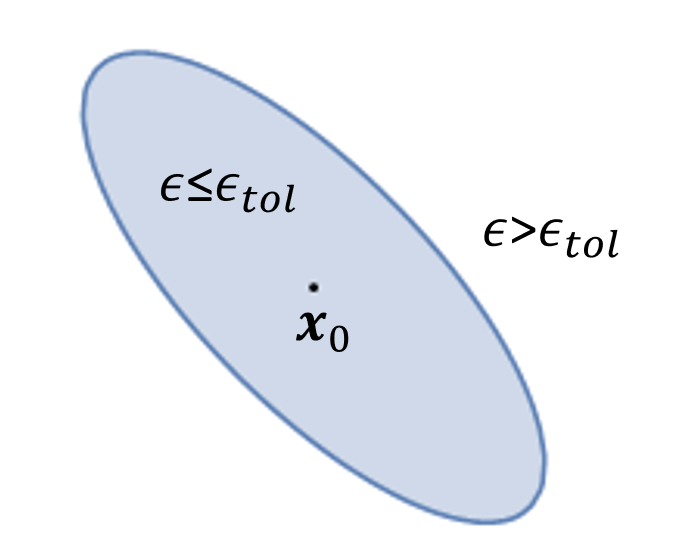
\includegraphics[width=0.20\linewidth]{Region of accuracy.png} 
\caption{Sketch of region of accuracy (ROA).}
\label{ISAT_ROA} 
\end{figure}
For initial setting, the linear term $\left.\frac{\partial  \mathbf{F}}{\partial \mathbf{x}}\right|_{\mathbf{x}_0}\cdot\left(\mathbf{x}-\mathbf{x}_0\right)$ is considered as an error. So, the initial $\mathbf{M}$ can be set as 
$$\mathbf{M}=\left(\left.\frac{\partial  \mathbf{F}}{\partial \mathbf{x}}\right|_{\mathbf{x}_0}\right)^T \left(\left.\frac{\partial  \mathbf{F}}{\partial \mathbf{x}}\right|_{\mathbf{x}_0}\right)/\epsilon_{tol}^2.$$


\begin{figure}[htbp]
\centering
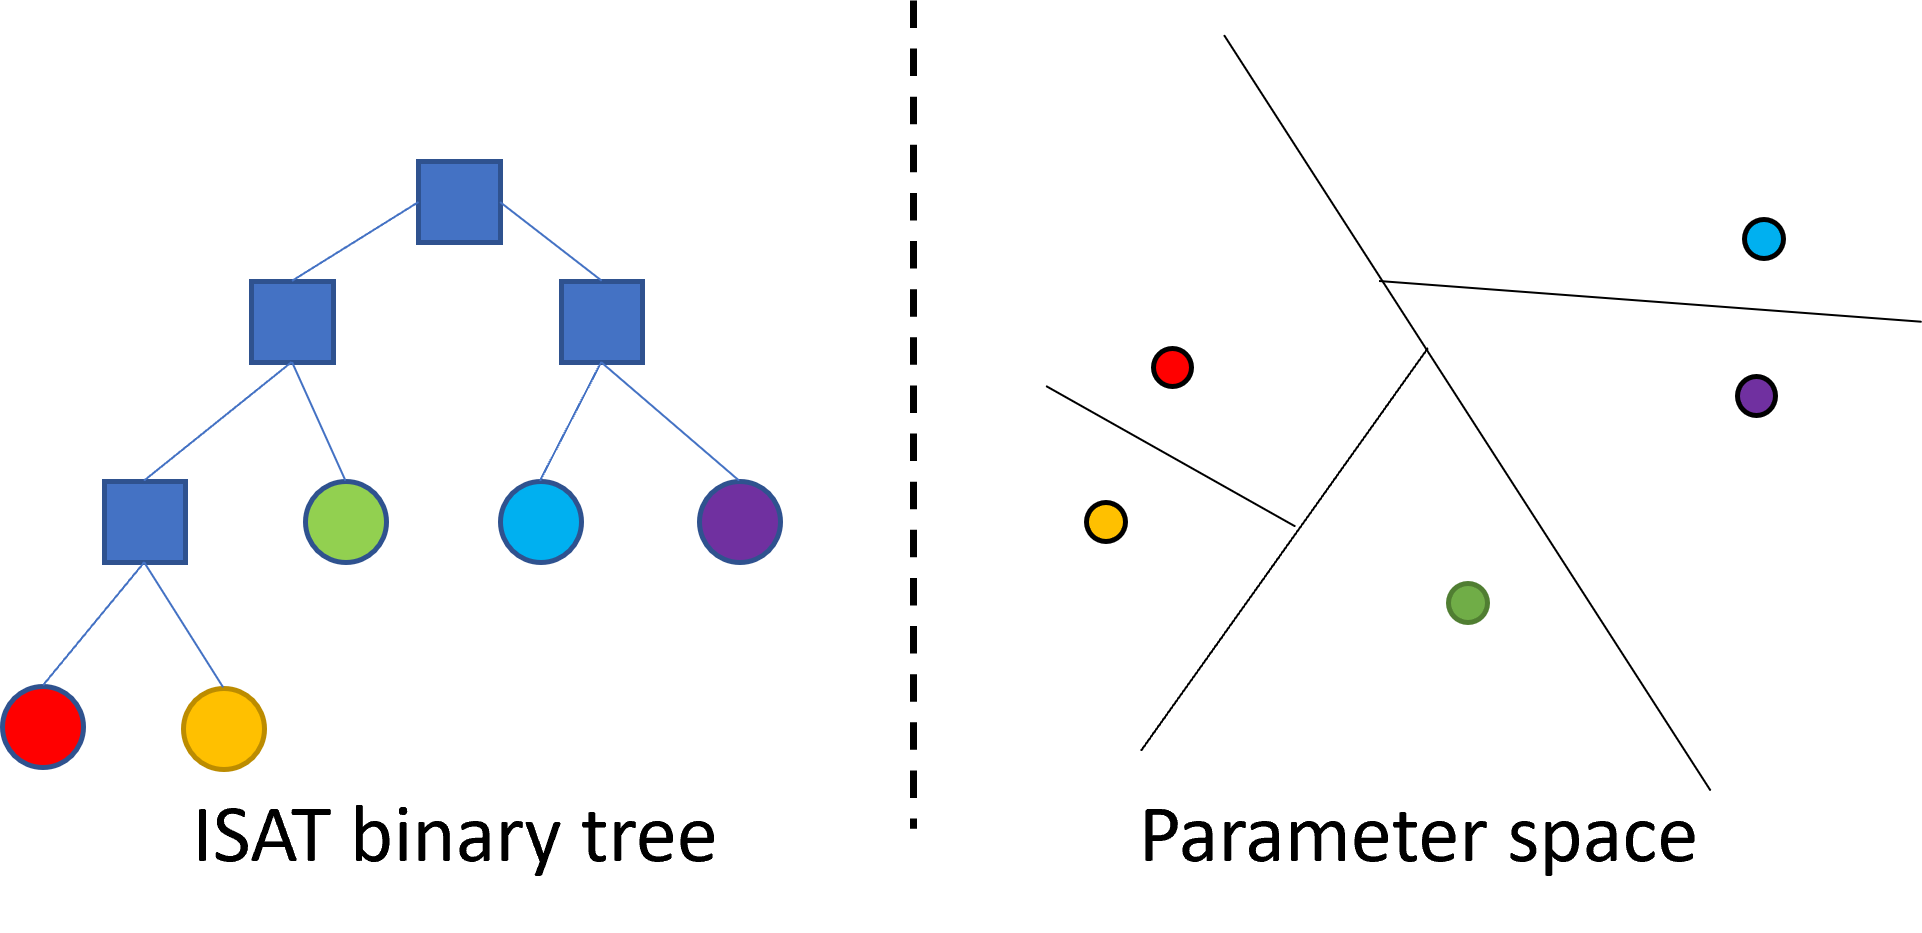
\includegraphics[width=0.6\linewidth]{ISAT tree.png}
\caption{The binary tree used to manage records in ISAT}
\label{ISAT_tree} 
\end{figure}
The management of records in the ISAT method is facilitated through a binary tree structure, as illustrated in Fig.~\ref{ISAT_tree}. Each node of the tree stores a vector that defines a hyperplane, dividing the parameter space into two distinct half-spaces. The data corresponding to each half-space is stored in the respective sub-trees. By employing this tree structure, the entire parameter space can be divided into numerous small cells, with the records being stored at the leaf nodes. During the search operation, at each layer of the tree, the sub-tree is selected based on which half-space contains the input parameter. This process continues until the desired record is found. It is important to note that the record obtained through this method may not be the closest to the input data. Nevertheless, this approach is simple and efficient enough to satisfy the requirements of the simulation. When it comes to the insertion operation, a new node is created, and its hyperplane is defined using the median plane of a table record (obtained from the search operation) and the record being inserted. The ISAT binary tree is not a balanced tree.  Consequently, during simulations, a large number of records may be concentrated in one of the two sub-trees, resulting in an increased height of the tree structure. This can negatively impact the performance of lookup and insertion operations. To prevent such degradation, a rebuilding process is implemented. Specifically, at every 20 time steps, if the tree height exceeds twice the height of a perfectly balanced tree, a new tree structure is constructed using the existing records to restore perfect balance and optimize performance.



In a simulation, for the first query, a new record is calculated and added to the table. 
For subsequent queries $(\mathbf{x}_{new})$, the closest record $(\mathbf{x}_0,\mathbf{y}_0,\left.\frac{\partial \mathbf{F}}{\partial \mathbf{x}}\right|_{\mathbf{x}_0}, \mathbf{M})$ is searched out, and then one of the following three operations is conducted, as shown in Fig.~\ref{ISAT_ALG}:

(1) \textbf{Retrieval}: If $\mathbf{x}_{new}$ is within the EOA of the record, then the linear approximation $\mathbf{y}_{linear}$ is returned. Otherwise $\mathbf{y}_{new}=\mathbf{F}\left(\mathbf{x}_{new}\right)$ is calculated. 

(2) \textbf{Growth}: If $\left|\mathbf{y}_{new}- \mathbf{y}_{linear}\right|\leq\epsilon_{tol}$, then EOA is grown to include $\mathbf{x}_{new}$. Specifically, the new EOA is the smallest ellipsoid covering both the old EOA and $\mathbf{x}_{new}$. $\mathbf{y}_{new}$ is returned.

(3) \textbf{Addition}: Otherwise $\left|\mathbf{y}_{new}- \mathbf{y}_{linear}\right|>\epsilon_{tol}$, then new record is added to the table, and $\mathbf{y}_{new}$ is returned.

\begin{figure}[htbp]
\centering
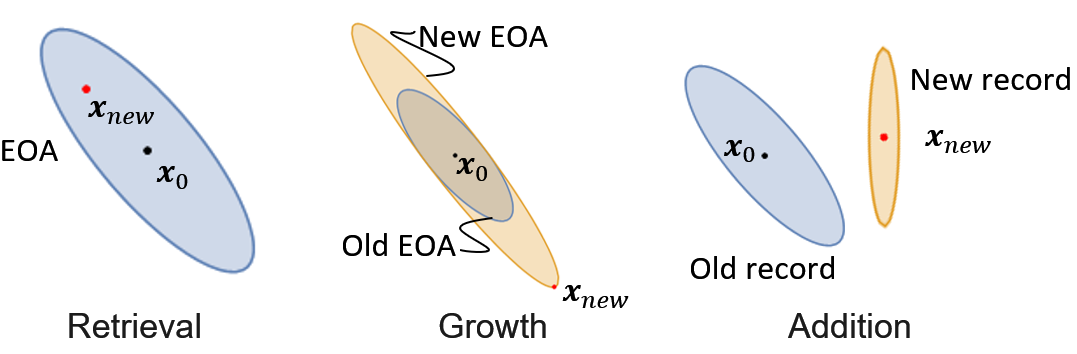
\includegraphics[width=0.6\linewidth]{s.png}
\caption{Sketch showing the three operations in the ISAT method.}
\label{ISAT_ALG} 
\end{figure}

In the ISAT method, a maximum number of records are set due to the limitation of memory. When the number of records reaches the maximum, the table is full, and new addition actions can't be taken. In L. Lu and S.B Pope's work \cite{lu2009improved}, they compared three actions: (a) don't add the new record to the table; (b) remove the least recently used record; (c) remove the least frequently used record. They claimed that for non-stationary problems, (b) is likely optimal. They maintain a linked list (called MFU list in \cite{lu2009improved}) to obtain the least recently used record. In the list, the records are in the order in which they have most frequently been used. We follow their idea (b) and further improve the method to remove records.

In our tests, we realized that the height of the binary tree becomes larger when there are more records, making the search slower. Moreover, in the non-stationary simulation, a large number of records are required only in a certain time interval, after which many records are redundant and only degrade the performance of the search. These redundant records should be accurately detected and quickly deleted to improve performance. We propose two methods, 
\begin{itemize}
\item delete data that has not been used in the last few time steps. 
\item use an adaptive table maximum size, and the size is formulated as:
\end{itemize}
\begin{align}
N_{max} = C \sum_{i=0}^M  N_{\text{inactive},i}  \label{eq:adap}
\end{align}
where $ N_{\text{inactive},i}$ is the number of records of which the last call was $i$ time steps ago. $M$ is the number of time steps considered and $C$ is a multiplier ($C>1$). $M$ and $C$ are tunable parameters.


We propose a new data structure to support the proposed methods. The data structure is a list of linked lists, shown in Fig.~\ref{ISAT_LL}. It has multiple layers (4 layers in Fig.~\ref{ISAT_LL}), $T_1$ stores the records just used in the previous time step, $T_2$ stores the records used in the time step before the previous time step, and so on and so forth. $T_4$ has all records not been used within 3 latest time steps. With this list, all records are sorted according to the distance between the current time step and the time step of the last call, and the proposed deletion methods can be efficiently implemented. The main list ($T_1-T_4$ list) is a circular array, the list head is the layer of the most recently used records and the tail is the layer of the least recently used records. In a new time step, the linked list of the tail ($T_4$) is merged with the previous layer ($T_3$), and this empty layer ($T_4$) becomes the new head, and all records called during this time step will insert into this layer. The previous layer ($T_3$) becomes the new tail. Since we use a combination of a circular array and linked lists, the above operations can be accomplished achieved with O(1) time complexity.

\begin{figure}[htbp]
\centering
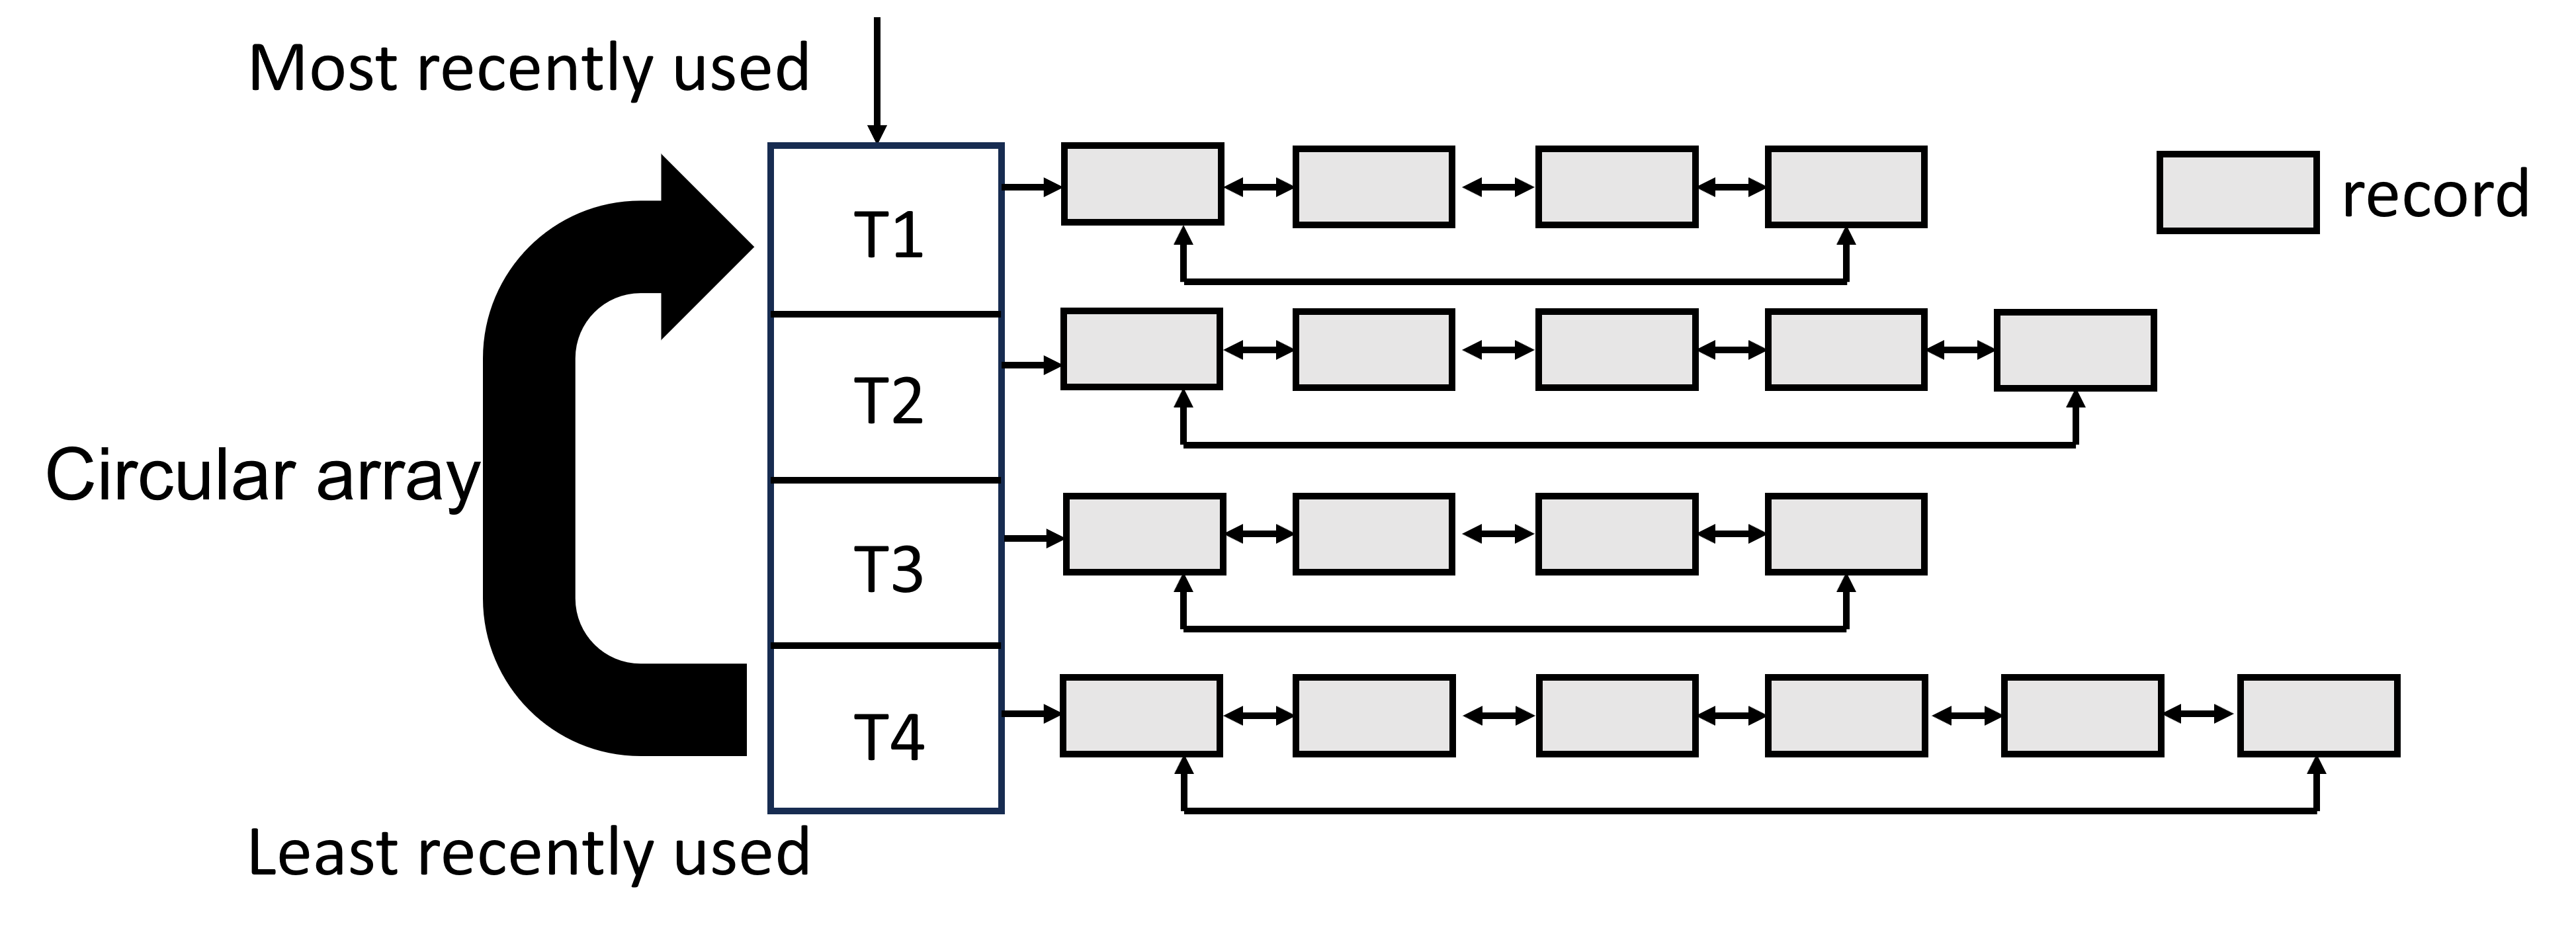
\includegraphics[width=0.6\linewidth]{linkedlist2.png}
\caption{schematic of the data structure to support methods for removing redundant records}
\label{ISAT_LL} 
\end{figure}

\subsection{Analytical framework for VLE}
\label{sec:analytical}

The first-order derivatives of thermodynamic properties considering phase change are required when calculating the speed of sound (Eq.~\ref{eq:soundspeed}), solving the VLE system (e.g., using the Newton-Raphson iteration method), and using the ISAT-VLE method (e.g., evaluating the Jacobian matrix $\left.\frac{\partial  \mathbf{F}}{\partial \mathbf{x}}\right|_{\mathbf{x}_0}$). These derivatives can be obtained numerically by a perturbation method, which is more computationally expensive and introduces additional errors. Most importantly, profiles of thermodynamic properties can have discontinuities/jumps at the phase boundaries, and hence the numerical derivatives from the perturbation method can be incorrect and diverge the simulation. To address all the above challenges, We developed an analytical method to evaluate the required derivatives.
In order to calculate the derivatives of thermodynamic properties considering phase change, after obtaining a few derivatives listed below, the calculation can be finished using a simple framework.
\begin{align}
\left(\frac{\partial x_k}{\partial T}\right)_{P,\mathbf{z}},\left(\frac{\partial y_k}{\partial T}\right)_{P,\mathbf{z}},\left(\frac{\partial x_k}{\partial P}\right)_{T,\mathbf{z}},\left(\frac{\partial y_k}{\partial P}\right)_{T,\mathbf{z}},\left(\frac{\partial x_k}{\partial z_i}\right)_{T,P,z_{s,s\neq i}},\left(\frac{\partial y_k}{\partial z_i}\right)_{T,P,z_{s,s\neq i}}
\end{align}
The formula of these terms is provided in Appendix ~\ref{App:VLE}, and its derivation is based on Tudisco and Menon's work \cite{tudisco2020analytical}.
For single-phase properties, the temperature and pressure derivatives can be obtained using the chain rule:
\begin{align}
\left(\frac{\partial (\cdot)_l}{\partial T}\right)_{P,\mathbf{z}} = \left(\frac{\partial (\cdot)_l}{\partial T}\right)_{P,\mathbf{x}} + \sum_{k=1}^N\left(\frac{\partial (\cdot)_l}{\partial x_k}\right)_{P,T,x_{s,s\neq k}}\left(\frac{\partial x_k}{\partial T}\right)_{P,\mathbf{z}} \label{eq:dvdT}
\end{align}
\begin{align}
\left(\frac{\partial (\cdot)_v}{\partial T}\right)_{P,\mathbf{z}} = \left(\frac{\partial (\cdot)_v}{\partial T}\right)_{P,\mathbf{y}} + \sum_{k=1}^N\left(\frac{\partial (\cdot)_v}{\partial y_k}\right)_{P,T,y_{s,s\neq k}}\left(\frac{\partial y_k}{\partial T}\right)_{P,\mathbf{z}} \label{eq:dldT}
\end{align}
The pressure derivatives use similar formulas with all the $\left(\frac{\partial (\cdot)}{\partial T }\right)$ replaced by $\left(\frac{\partial (\cdot)}{\partial P }\right)$.

The $z$ derivatives are formulated as:
\begin{align}
\left(\frac{\partial (\cdot)_l}{\partial z_i}\right)_{P,T} =  \sum_{k=1}^N\left(\frac{\partial (\cdot)_l}{\partial x_k}\right)_{P,T,x_{s,s\neq k}}\left(\frac{\partial x_k}{\partial z_i}\right)_{P,T,\mathbf{z}} \label{eq:dldz}
\end{align}

\begin{align}
\left(\frac{\partial (\cdot)_v}{\partial z_i}\right)_{P,T} =  \sum_{k=1}^N\left(\frac{\partial (\cdot)_v}{\partial x_k}\right)_{P,T,x_{s,s\neq k}}\left(\frac{\partial y_k}{\partial z_i}\right)_{P,T,\mathbf{z}} \label{eq:dvdz}
\end{align}

Note that the derivatives such as $\left(\frac{\partial (\cdot)_v}{\partial T}\right)_{P,\mathbf{y}}$,$\left(\frac{\partial (\cdot)_v}{\partial P}\right)_{T,\mathbf{y}}$, $\left(\frac{\partial (\cdot)_v}{\partial y_k}\right)_{P,T,y_{s,s\neq k}}$, are single-phase derivatives, and no phase change calculation is involved. These terms can be directly obtained by taking derivatives of the analytical form of EOS (including the departure functions derived from EOS) and NASA Polynomials. 


In TP flash, the thermodynamic properties are considered as a function of mixture temperature $T$, pressure $P$, and composition $\mathbf{z}$. The first-order derivatives are required by TP flash calculation (e.g., using the Newton-Raphson iteration method) and also the ISAT of TP flash solutions (e.g., evaluating the Jacobian matrix $\left.\frac{\partial  \mathbf{F}}{\partial \mathbf{x}}\right|_{\mathbf{x}_0} = \left.\frac{\partial  \left(\rho, e, \beta, c\right)}{\partial \left(P,T,\mathbf{z}\right)}\right|_{\mathbf{x}_0}$).
First, the derivative of $\beta$ is formulated as: (details are shown in Appendix~\ref{App:VLE})

\begin{align}
\left(\frac{\partial \beta }{\partial T}\right)_{P,\mathbf{z}} = \sum_{k=1}^N \left(\frac{\partial v_k}{\partial T}\right)_{P,\mathbf{z}},\left(\frac{\partial \beta}{\partial P}\right)_{T,\mathbf{z}} = \sum_{k=1}^N \left(\frac{\partial v_k}{\partial P}\right)_{T,\mathbf{z}}, \left(\frac{\partial \beta}{\partial z_i}\right)_{T,P,z_{s,s\neq i}}=\sum_{j=1}^N\left(\frac{\partial N_{j,v}}{\partial N_i}\right)_{T,P,N_{s,s\neq j}} -\beta
\end{align}
where $v_k$ is the mole fraction of component $k$ in the vapor phase of the total mixture ($v_k = \beta y_k$), 
$N_i$ is the total number of moles of component $i$ in the mixture, and $N_{k,v}$ are the number of moles of component $k$ in vapor phase.

The derivative of $\rho$ and $e$ are obtained from Eq.~\ref{eq:rho} and Eq.~\ref{eq:e}.
\begin{align}
\left(\frac{\partial \rho}{\partial T} \right)_{P,\mathbf{z}}= 
- \frac{\rho^2}{M}\Bigg\{\left(\frac{\partial \beta}{\partial T}\right)_{P,\mathbf{z}}\left(\frac{M_v}{\rho_v}-\frac{M_l}{\rho_l}\right) + 
\frac{\beta}{\rho_v^2}\left[\rho_v\left(\frac{\partial M_v}{\partial T} \right)_{P,\mathbf{z}}-M_v \left(\frac{\partial \rho_v}{\partial T} \right)_{P,\mathbf{z}}\right] \\+
\frac{1-\beta}{\rho_l^2}\left[\rho_l\left(\frac{\partial M_l}{\partial T} \right)_{P,\mathbf{z}}-M_l \left(\frac{\partial \rho_l}{\partial T} \right)_{P,\mathbf{z}}\right]\Bigg\} 
\end{align}
\begin{align}
\left(\frac{\partial e}{\partial T}\right)_{P,\mathbf{z}}= \frac{1}{M}\left\{ \left(\frac{\partial \beta}{\partial T}\right)_{P,\mathbf{z}} \left(M_v e_v-M_l e_l\right)+\beta \left[e_v\left(\frac{\partial M_v}{\partial T}\right)_{P,\mathbf{z}}+M_v\left(\frac{\partial e_v}{\partial T}\right)_{P,\mathbf{z}}\right]\right.\\ \left.+\left(1-\beta\right)\left[e_l\left(\frac{\partial M_l}{\partial T}\right)_{P,\mathbf{z}}+M_l\left(\frac{\partial e_l}{\partial T}\right)_{P,\mathbf{z}}\right]\right\}
\end{align}
The derivatives of single phase properties such as $\left(\frac{\partial e_v}{\partial T}\right)_{P,\mathbf{z}}$,$\left(\frac{\partial M_v}{\partial T}\right)_{P,\mathbf{z}}$,$\left(\frac{\partial \rho_v}{\partial T} \right)_{P,\mathbf{z}}$, can be calculated using Eq.~\ref{eq:dvdT}-\ref{eq:dldT}. For the temperature derivatives, similar formulas can be used, with all the $\left(\frac{\partial (\cdot)}{\partial P}\right)_{T,\mathbf{z}}$ replaced by $\left(\frac{\partial (\cdot)}{\partial T}\right)_{P,\mathbf{z}}$.

Since  $\left(\frac{\partial M}{\partial z_i}\right)_{P,T} \neq 0 $, $z$ derivatives have different formula: 

\begin{align}
\left(\frac{\partial \rho}{\partial z_i} \right)_{P,T}= 
- \frac{\rho^2}{M}\Bigg\{\left(\frac{\partial \beta}{\partial z_i}\right)_{P,T}\left(\frac{M_v}{\rho_v}-\frac{M_l}{\rho_l}\right) + 
\frac{\beta}{\rho_v^2}\left[\rho_v\left(\frac{\partial M_v}{\partial z_i} \right)_{P,T}-M_v \left(\frac{\partial \rho_v}{\partial z_i} \right)_{P,T}\right] \\+
\frac{1-\beta}{\rho_l^2}\left[\rho_l\left(\frac{\partial M_l}{\partial z_i} \right)_{P,T}-M_l \left(\frac{\partial \rho_l}{\partial z_i} \right)_{P,T}\right]- \frac{M_i-M}{\rho}\Bigg\} 
\end{align}
\begin{align}
\left(\frac{\partial e}{\partial z_i}\right)_{P,T}= \frac{1}{M}\left\{ \left(\frac{\partial \beta}{\partial z_i}\right)_{P,T} \left(M_v e_v-M_l e_l\right)+\beta \left[e_v\left(\frac{\partial M_v}{\partial z_i}\right)_{P,T}+M_v\left(\frac{\partial e_v}{\partial z_i}\right)_{P,T}\right]\right.\\ \left.+\left(1-\beta\right)\left[e_l\left(\frac{\partial M_l}{\partial z_i}\right)_{P,T}+M_l\left(\frac{\partial e_l}{\partial z_i}\right)_{P,T}\right] - e \left(M_i-M\right)\right\}
\end{align}
The single phase properties derivatives such as $\left(\frac{\partial e_v}{\partial z_i}\right)_{P,T}$,$\left(\frac{\partial M_v}{\partial z_i}\right)_{P,T}$,$\left(\frac{\partial \rho_v}{\partial z_i} \right)_{P,T}$, can be calculated using Eq.~\ref{eq:dldz}-\ref{eq:dvdz}.

%\begin{align}
%\left(\frac{\partial M_v}{\partial P}\right)_{T,\mathbf{z}} = \sum_{k=1}^N\left(\frac{\partial v_i}{\partial P}\right)_{T,\mathbf{z}} \frac{M_i}{\beta} - \left(\frac{\partial \beta}{\partial P}\right)_{T,\mathbf{z}}\frac{M}{\beta}
%\end{align}
%where $M$ is the mixture molar mass. 

The last property, speed of sound, is formulated as
$c^2 = \frac{1}{\kappa_s\rho}$.
where $\kappa_s$ is the isentropic compressibility $\kappa_s = \kappa_T -T \alpha_p^2/\rho c_p$.  The isobaric expansivity $\alpha_p$ and isothermal compressibility $\kappa_T$ are defined as $\alpha_p=-\left(\frac{\partial \rho}{\partial T}\right)_{P,\mathbf{z}}/\rho$, $\kappa_T=\left(\frac{\partial \rho}{\partial P}\right)_{T,\mathbf{z}}/\rho $.
 Combining all these equations, the speed of sounds is formulated as: 

 \begin{align}
c = \frac{1}{\sqrt{\left(\frac{\partial\rho}{\partial P}\right)_{T,\mathbf{z}} - \frac{T}{\rho^2 } \left.\left(\frac{\partial\rho}{\partial T}\right)_{P,\mathbf{z}} \middle/ \left[\left(\frac{\partial e}{\partial T}\right)_{P,\mathbf{z}}- \frac{P}{\rho^2}\left(\frac{\partial \rho}{\partial T}\right)_{P,\mathbf{z}}\right]\right.}}, \label{eq:soundspeed}
\end{align}

The speed of sound depends on the first derivatives,and hence, its derivatives require the computation of second derivatives, which need very complex calculations. Because the derivative of sound speed is only used in the ISAT method to provide a better linear approximation, in fact, by setting its derivative to zero we can still use ISAT error control to obtain a sufficiently accurate solution


Based on the formulas of the ($T,P,\mathbf{z}$) system for the TP flash solver, the first derivatives of the ($\rho,P, \mathbf{z}$) system for the PV flash solver and the ($e,\rho, \mathbf{z}$) system for the UV flash solver can be derived using the chain rule. Specifically, for the ($\rho,P,\mathbf{z}$) system, a property $F$ is written as $F(\rho(T,P,z),P,z)$, calculating temperature derivative using chain rule gives $\left(\frac{\partial F} {\partial \rho}\right)_{P,\mathbf{z}}\left(\frac{\partial \rho}{\partial T}\right)_{P,\mathbf{z}}= \left(\frac{\partial F}{\partial T}\right)_{P,\mathbf{z}}$. Hence, the density derivative is:

\begin{align}
\left(\frac{\partial (\cdot)}{\partial \rho}\right)_{P,\mathbf{z}} =\left. \left(\frac{\partial (\cdot)}{\partial T}\right)_{P,\mathbf{z}} \middle/ \left(\frac{\partial \rho}{\partial T}\right)_{P,\mathbf{z}}\right.
\end{align}
To derive the pressure and $z_i$ derivatives, $\left(\frac{\partial T}{\partial P}\right)_{\rho,\mathbf{z}}$ is needed. Taking pressure derivative of constant density equation $\rho(T(P,z),P,z)=Const$ gives $\left(\frac{\partial T} {\partial P}\right)_{\rho,\mathbf{z}}\left(\frac{\partial \rho}{\partial T}\right)_{P,\mathbf{z}}+ \left(\frac{\partial \rho}{\partial P}\right)_{T,\mathbf{z}}=0$, and so, $\left(\frac{\partial T}{\partial P}\right)_{\rho,\mathbf{z}} = - \left(\frac{\partial \rho}{\partial P}\right)_{T,\mathbf{z}}/ \left(\frac{\partial \rho}{\partial T}\right)_{P,\mathbf{z}}$
Taking pressure and $z_i$ derivative of $F(\rho(T,P,z),P,z)$ and substituting $\left(\frac{\partial T}{\partial P}\right)_{\rho,\mathbf{z}}$ into the results gives:
\begin{align}
\left(\frac{\partial (\cdot)}{\partial P}\right)_{\rho,\mathbf{z}} = \left.-\left(\frac{\partial (\cdot)}{\partial T}\right)_{P,\mathbf{z}} \left(\frac{\partial \rho}{\partial P}\right)_{T,\mathbf{z}}\middle/ \left(\frac{\partial \rho}{\partial T}\right)_{P,\mathbf{z}}+
\left(\frac{\partial (\cdot)}{\partial P}\right)_{T,\mathbf{z}}\right.
\end{align}
\begin{align}
\left(\frac{\partial (\cdot)}{\partial z_i}\right)_{P,\rho} = \left.-\left(\frac{\partial (\cdot)}{\partial T}\right)_{P,\mathbf{z}} \left(\frac{\partial \rho}{\partial z_i}\right)_{T,P,z_{j, j \neq i}}\middle/ \left(\frac{\partial \rho}{\partial T}\right)_{P,\mathbf{z}}+
\left(\frac{\partial (\cdot)}{\partial z_i}\right)_{T,P,z_{j, j \neq i}}\right.
\end{align}
For ($e,\rho,\mathbf{z}$) system, because the Jacobian matrix of ($e,\rho,\mathbf{z}$) and ($T,P,\mathbf{z}$) has the relation $\frac{\partial (e,\rho,\mathbf{z})}{\partial(T,P,\mathbf{z})}\frac{\partial(T,P,\mathbf{z})}{\partial (e,\rho,\mathbf{z})} = I$, $I$ is the identity matrix. The derivative of any property $F$ in  ($e,\rho,\mathbf{z}$) system can be obtained by $\frac{\partial F}{\partial (e,\rho,\mathbf{z})}=\frac{\partial F}{\partial(T,P,\mathbf{z})}\frac{\partial(T,P,\mathbf{z})}{\partial (e,\rho,\mathbf{z})} = \frac{\partial F}{\partial(T,P,\mathbf{z})} \frac{\partial (e,\rho,\mathbf{z})}{\partial(T,P,\mathbf{z})}^{-1}$
Calculating the inverse matrix gives:
\begin{align}
\Delta = \left(\frac{\partial e}{\partial T}\right)_{P,\mathbf{z}} \left(\frac{\partial \rho}{\partial P}\right)_{T,\mathbf{z}} - 
\left(\frac{\partial e}{\partial P}\right)_{T,\mathbf{z}} \left(\frac{\partial \rho}{\partial T}\right)_{P,\mathbf{z}}
\end{align}
\begin{align}
\left(\frac{\partial (\cdot)}{\partial e}\right)_{\rho,\mathbf{z}} = \frac{1}{\Delta}\left[
\left(\frac{\partial (\cdot)}{\partial T}\right)_{P,\mathbf{z}}
\left(\frac{\partial \rho}{\partial P}\right)_{T,\mathbf{z}}  -
\left(\frac{\partial (\cdot)}{\partial P}\right)_{T,\mathbf{z}}
\left(\frac{\partial \rho}{\partial T}\right)_{P,\mathbf{z}} \right]
\end{align}
\begin{align}
\left(\frac{\partial (\cdot)}{\partial \rho}\right)_{e,\mathbf{z}} = \frac{1}{\Delta}\left[-
\left(\frac{\partial (\cdot)}{\partial T}\right)_{P,\mathbf{z}}
\left(\frac{\partial e}{\partial P}\right)_{T,\mathbf{z}}  +
\left(\frac{\partial (\cdot)}{\partial P}\right)_{T,\mathbf{z}}
\left(\frac{\partial e}{\partial T}\right)_{P,\mathbf{z}} \right]
\end{align}

\begin{align}
\left(\frac{\partial (\cdot)}{\partial z_i}\right)_{e,\rho,z_{j,j\neq i}} = \left(\frac{\partial (\cdot)}{\partial z_i}\right)_{T,P,z_{j,j\neq i}} + \left(\frac{\partial (\cdot)}{\partial T}\right)_{P,\mathbf{z}} \left(\frac{\partial T}{\partial z_i}\right)_{e,\rho,z_{j,j\neq i}} + 
\left(\frac{\partial (\cdot)}{\partial P}\right)_{T,\mathbf{z}}
\left(\frac{\partial P}{\partial z_i}\right)_{e,\rho,z_{j,j\neq i}}
\end{align}
\begin{align}
\left(\frac{\partial T}{\partial z_i}\right)_{e,\rho,z_{j,j\neq i}} = \frac{1}{\Delta}\left[-
\left(\frac{\partial \rho}{\partial P}\right)_{T,\mathbf{z}}
\left(\frac{\partial e}{\partial z_i}\right)_{e,\rho,z_{j,j\neq i}}  +
\left(\frac{\partial e}{\partial P}\right)_{T,\mathbf{z}}
\left(\frac{\partial \rho}{\partial z_i}\right)_{e,\rho,z_{j,j\neq i}} \right]
\end{align}

\begin{align}
\left(\frac{\partial P}{\partial z_i}\right)_{e,\rho,z_{j,j\neq i}} = \frac{1}{\Delta}\left[]
\left(\frac{\partial \rho}{\partial T}\right)_{T,\mathbf{z}}
\left(\frac{\partial e}{\partial z_i}\right)_{e,\rho,z_{j,j\neq i}}  -
\left(\frac{\partial e}{\partial T}\right)_{T,\mathbf{z}}
\left(\frac{\partial \rho}{\partial z_i}\right)_{e,\rho,z_{j,j\neq i}} \right]
\end{align}


\section{Numerical test}
\subsection{Transcritical temporal mixing layer (TML)}
\label{sec:TML}

In this section, a series of high-pressure transcritical temporal mixing layer (TML) cases are simulated using our VLE-based CFD solver. The simulations are conducted to investigate the ISAT-VLE method performance when resolving the important shearing effect in jet flows. The schematic of the transcritical TML configuration is shown in Fig.~\ref{TML_GEO}. The computational domain is a rectangular box of size $L_x \times L_y \times L_z$.
The upper half is filled with n-dodecane (\ce{n-C12H26}) which flows to the right with the velocity $U_T$, and the lower half is filled with \ce{N2} which flows to the left with the velocity $U_B$. In the vertical $z$ direction, the domain is split into 3 subdomains: $L_z = L_{buff}+L_{TML}+L_{buff}, L_{buff} = L_{TML} = 1/3 L_z$. The focus of this simulation is on TML evolution in the center cubic subdomain $L_x \times L_y \times L_{TML}$. The center subdomain is uniformly discretized in all directions (256 × 152 × 256), the top and bottom subdomain have a stretched grid along the z direction (256 × 152 × 64, aspect ratio close to the center subdomain: 1.01, aspect ratio at top and bottom boundary: 10.1). The configuration is the same as that in Miller et al. \cite{miller2001direct}. The initial cross-stream mean profiles, including velocity, temperature, and mass fractions, are set using an error function profile: $\textrm{erf}(\sqrt{\pi}z/\delta_{\omega,0})$, where $\delta_{\omega,0}$ is the initial vorticity layer thickness. The stream-wise velocity is determined using the condition of stationary vortices (Eq.~\ref{eq:initU}), which is derived by Miller et al. \cite{miller2001direct} to obtain stationary vortices in temporal mixing layer simulation. Since the condition of stationary vortices is derived under the assumption of calorically perfect gases, vortices don't stay truly stationary for real gas simulations.
\begin{align} U_T = \frac{2M_c c_T}{1+\sqrt{\gamma_T/\gamma_B}},U_B = -U_T \frac{c_B}{c_T}\sqrt{\gamma_T/\gamma_B} \label{eq:initU} \end{align}

where $M_c$ is the convective Mach number, and $M_c$ is fixed to 0.3 in the present research; $\gamma$ and $c$ are the heat capacity ratio and speed of sound, respectively. 
The simulations are conducted on a domain with $L_x = 4 \lambda_x = 29.16 \delta_{\omega,0}$, $L_y = 0.6 L_x$, and $L_{TML}=L_x$. 
The initial Reynolds number is defined as $Re_0 = [0.5(\rho_U +\rho_L)\Delta_{U_0} \delta_{\omega,0}]/\mu,\mu = 0.5 (\mu_T+\mu_B)$.
%Since this condition is derived under calorically perfect gases assumption, this condition can't guarantee a stationary vortex.

% the fine mesh $256\times 152 \times 256$ is used, and for course mesh it is $256\times 152\times 64$. The initial condition is set using the method used in \cite{masi2013multi}.  The initial Reynolds number is defined as $Re = [0.5(\rho_U +\rho_L)\Delta_{U_0} \delta_0]/\mu_R$, The $U_T$ and $U_B$ are defined as: 
The TML configuration sets periodic boundary conditions along the streamwise ($x$) and spanwise ($y$) direction, and the non-reflective outflow condition is used along crosswise ($z$) direction (in Fig.~\ref{TML_GEO}). A velocity perturbation is superimposed to trigger the instability, and the velocity perturbation was derived in Masi et al. \cite{masi2013multi}. The velocity perturbation in the $x-z$ plane is:
$$ a_1 = \frac{1}{4} e^{\pi (\delta_{\omega,0}/ \lambda_{xi})^2}(\textrm{erf}(\sqrt{\pi}(z/\delta_{\omega,0}+ \delta_{\omega,0}/\lambda_{xi}))-1);$$
$$ a_2 = -\frac{1}{4} e^{\pi (\delta_{\omega,0}/ \lambda_{xi})^2}(\textrm{erf}(\sqrt{\pi}(z/\delta_{\omega,0}- \delta_{\omega,0}/\lambda_{xi}))+1);$$
$$u_x = F_{2D} \Delta U \sum_i A_i sin(2\pi x/ \lambda_{xi}) (-a_1 e^{2\pi z / \lambda_{xi}}+a_2 e^{- 2\pi z / \lambda_{xi}});$$
$$u_z= F_{2D} \Delta U \sum_{i=0}^{2} A_i cos(2\pi x/ \lambda_{xi}) (-a_1 e^{2\pi z / \lambda_{xi}}+a_2 e^{- 2\pi z / \lambda_{xi}}),$$
where $\Delta U = |U_T-U_B|$, and $\lambda_{xi}=2^i\lambda_x$. $F_{2D}, A_i$ are coefficients to determine the perturbation magnitude \cite{masi2013multi}. The velocity perturbation in the y-x plan uses the same form, but replacing $\lambda_x$ by $\lambda_y = 0.6 \lambda_x$. Its perturbation magnitude ($z$ direction) are controlled using $F_{3D}, B_i$. The initial conditions for the two simulation cases in present study are shown in Table ~\ref{TML_init_table}.

\begin{figure}[htbp]
\centering

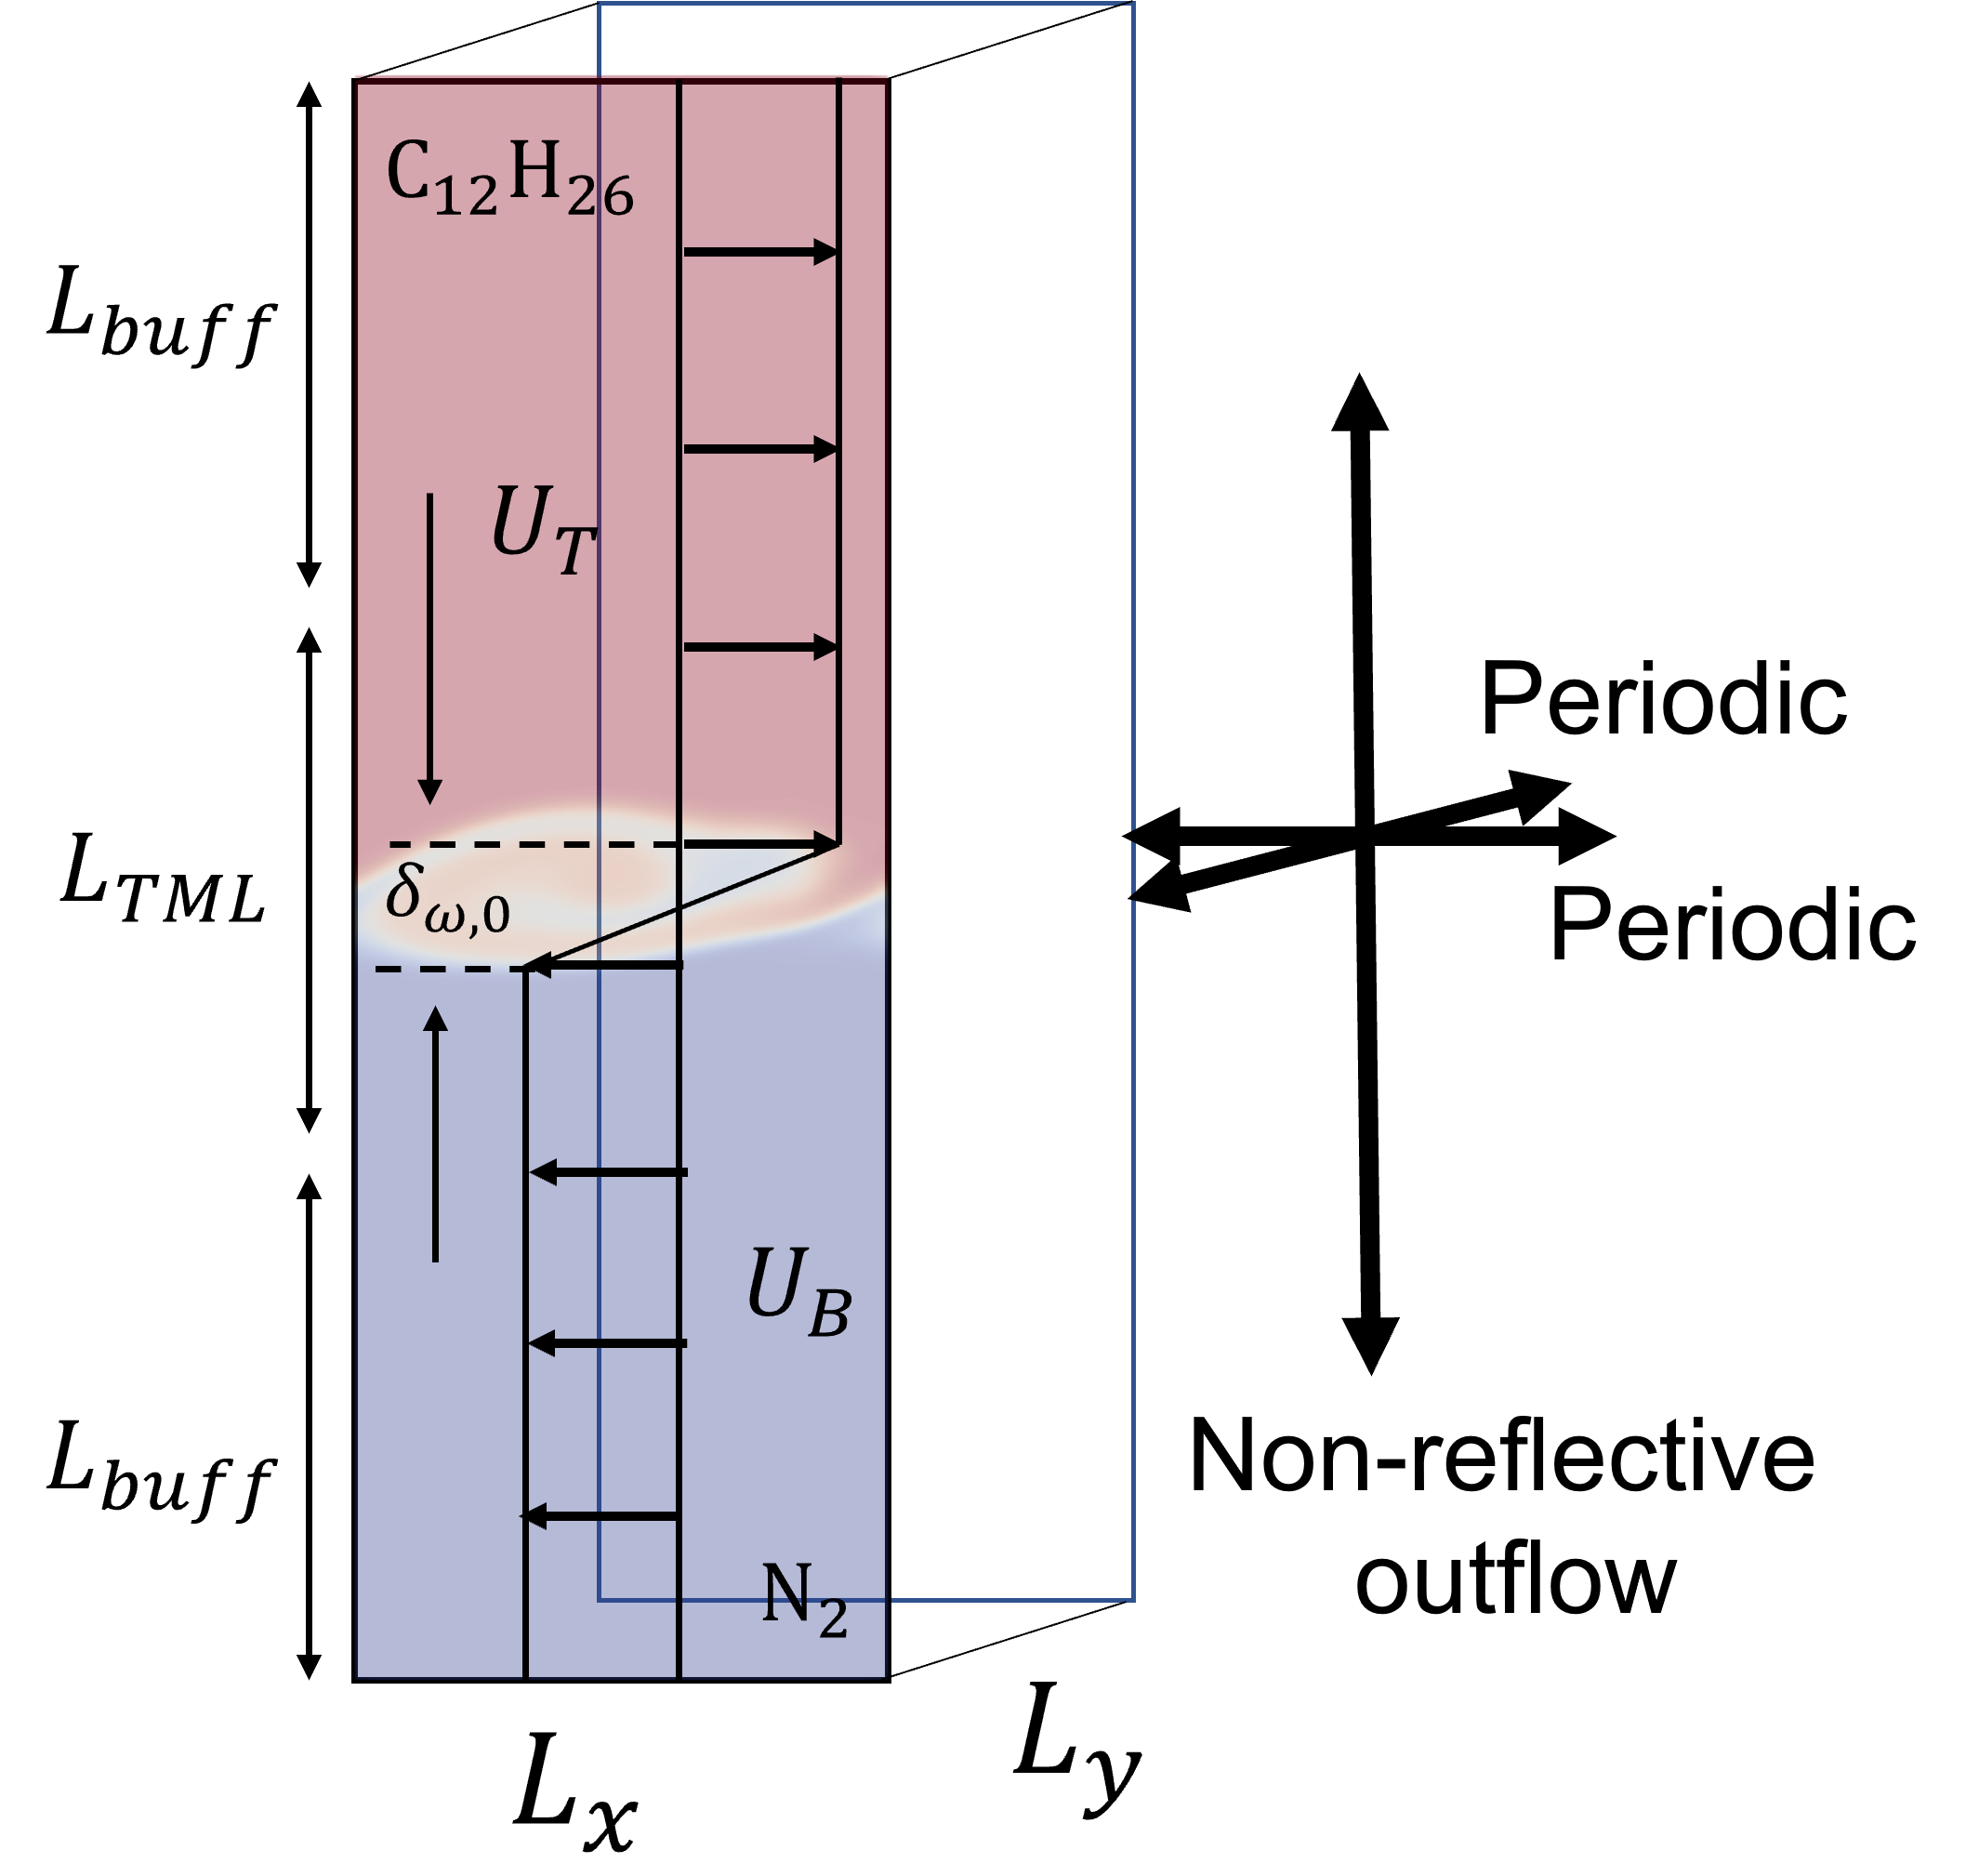
\includegraphics[width=0.45\linewidth]{TML_sc.png}
\hspace{.2in}
\raisebox{0.1\height}{
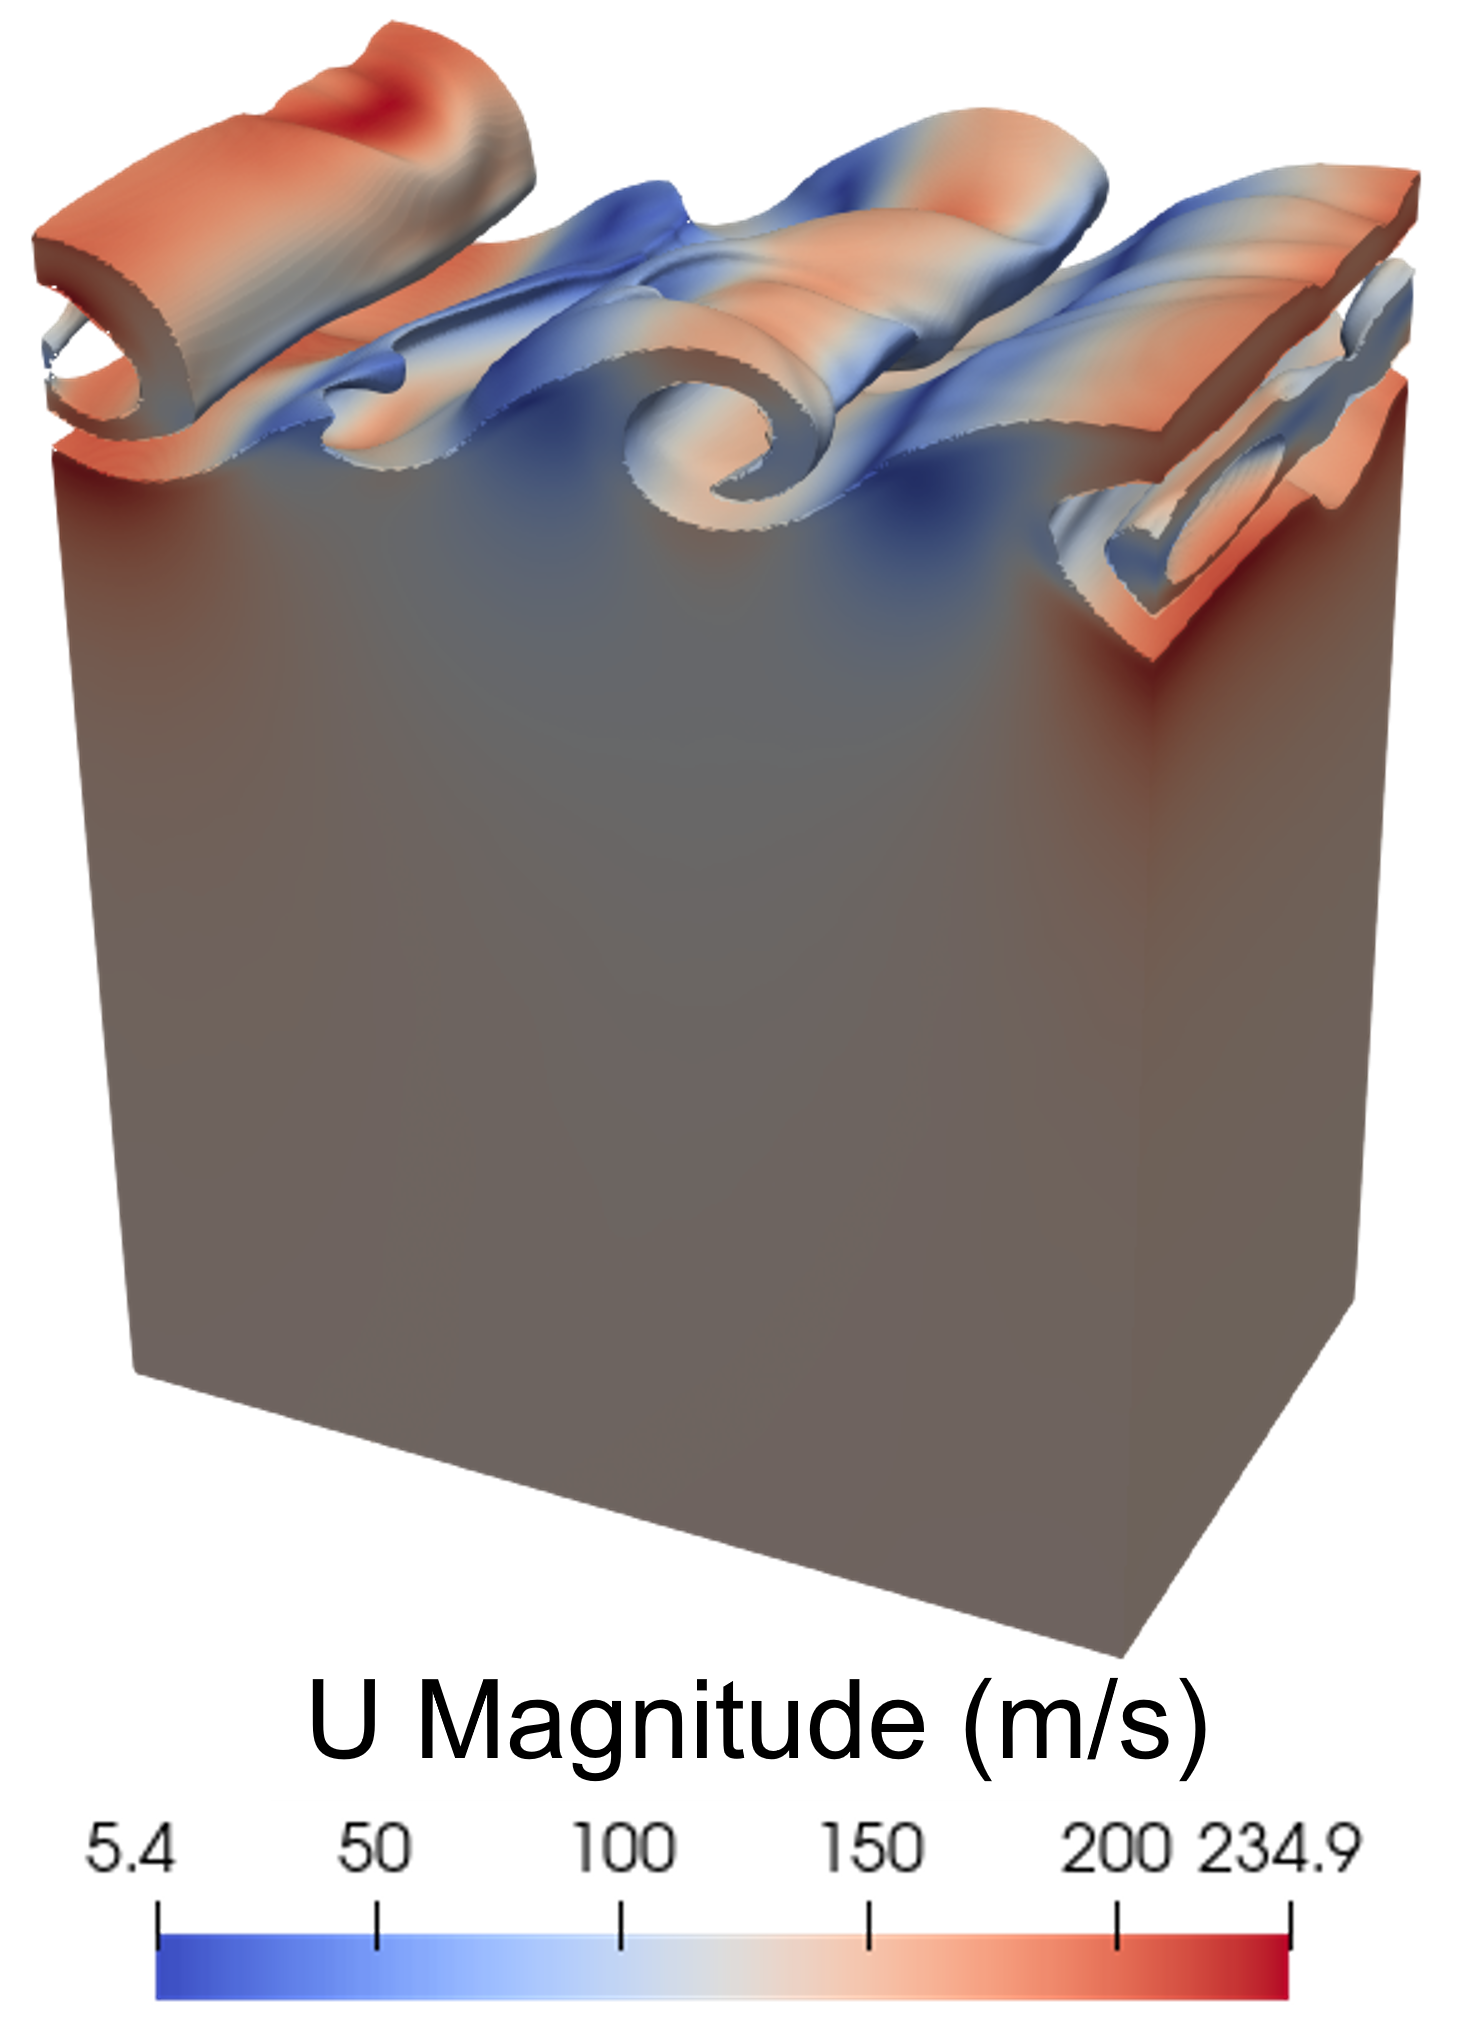
\includegraphics[width=0.25\linewidth]{3D_sc_s2.png}}
\caption{Left: Configuration of transcritical temporal mixing layer (TML) simulations. Right: 3D VLE-based CFD simulation of the transcritical TML, $t=2\times 10^-7s$, iso-surface: mass fraction of n-dodecane $Y_{C_{12}H_{26}} = 0.3$, color: velocity magnitude.}
\label{TML_GEO} 
\end{figure}



\begin{table}
    \caption{The initial condition of temporal mixing layer.}\label{TML_init_table}
    \begin{threeparttable} 
\begin{tabular*}{0.8\textwidth}{@{} l|lllll@{}}
    \toprule
    Properties     & $U_T (m/s)$   & $U_B (m/s)$  & $T_T (K)$   & $L_x (m)$ & $\delta_{\omega_0}$\\
    \midrule
    Case 1         & 77.94         & 134.27       & 600         & $2.79 \times 10^{-5}$   & $9.58 \times 10^{-7}$   \\
    Case 2         & 59.67         & 89.01        & 800         & $3.55 \times 10^{-5}$   & $1.22\times 10^{-6}$    \\
    \bottomrule
\end{tabular*}
\begin{tablenotes}
    \footnotesize    
    \item Subscripts T and B refer to Top and Bottom, respectively. $L_y = 0.6\times L_x$,  $Re_0=1000$. Mesh in the center subdomain is $256\times 152 \times 256$, and the top and bottom subdomain mesh is $256\times 152\times 64$. $P = 50$ bar, $T_B=293$ K, $M_c = 0.3$, $A_i = 0.25, 0.5, 1$, $B_i = 0.05, 0, 1$, and $F_{2D}= F_{3D} = 0.05$.\\
  \end{tablenotes}
\end{threeparttable}
\end{table}



\subsubsection{ISAT-VLE's performance and error control in 2D simulations:}





%First, 2D simulations are conducted to test ISAT performance and error control. 
In this subsection, we utilize the configuration of Case 1 in Table.~\ref{TML_init_table}. For 2D simulation, and the velocity in the y direction is set to zero. A set of error tolerance values are employed to assess the performance.  Using the FC method, the ISAT-VLE approach provides pressure, temperature, vapor fraction, and speed of sound results. The parameter $k$ is utilized to adjust the error tolerance, where the error tolerance $(T_{tol},p_{tol},\beta_{tol},c_{tol})= k (10^2, 10^6, 1, 10^2)$. This error tolerance is defined based on the magnitude of the properties, hence $k$ can be roughly considered as a maximum relative error. in which the order of magnitude of the tolerances depends on the magnitude of the properties. Hence, $k$ can be roughly considered as a maximum relative error. The simulation is run to $2\times 10^{-7}$ s to capture the vortex formation process from a flat interface under the influence of initial perturbation. 

Fig.~\ref{TML_PE}(a) illustrates the performance of the ISAT-VLE method. The blue dotted line represents the CPU time consumed by all other models in the CFD solver, which is significantly lower than the time consumed by the VLE model. Without the ISAT method, the VLE model accounts for 92.9\% of the CPU resources.The other curves in Fig.~\ref{TML_PE}(a) depict the accelerated performance of the VLE model with ISAT for different $k$ values (error tolerances), where a larger tolerance yields better performance. At the initial stage, the ISAT-VLE model runs approximately 15-61 times faster than the original VLE model, and in the final stage, it achieves a speed-up factor of 4-24. This is because the CPU time for all ISAT-VLE results increases as the mixing process generates more thermodynamic states. The performance curves of the ISAT-VLE results exhibit oscillation, which is attributed to the re-balancing of the binary tree when the overall structure becomes highly unbalanced (Sec.~\ref{sec:ISAT}). Simulations with larger tolerances exhibit shorter CPU times in each step, making the influence of re-balancing on performance (oscillation) more pronounced.


Fig.~\ref{TML_PE}(b) showcases the error control of the ISAT-VLE method. The errors presented in the plot are from the simulation with $k= 3 \times 10^{-3}$. The error is normalized by the tolerance, and the dashed line indicates that the error is equal to the tolerance ($\text{normalized error}=1$). The average error is evaluated using $\frac{\sum_i |e_i|V_i}{\sum_i V_i}$, where $V_i$ is cell volume, $e_i$ error in cell $i$. The average error is controlled to be 2 to 3 orders of magnitude smaller than the tolerance. Although the maximum error can exceed the tolerance, it remains within a similar order of magnitude. Table~\ref{TML_FC_table} shows the absolute and relative errors for all cases. As the tolerance decreases, the error is better controlled. For this particular simulation, $k= 3 \times 10^{-3}$ proves to be a suitable choice, ensuring pressure and temperature errors are kept within 0.5\% while achieving a total speed-up factor of 8.5.



\begin{figure}[htbp]
\centering
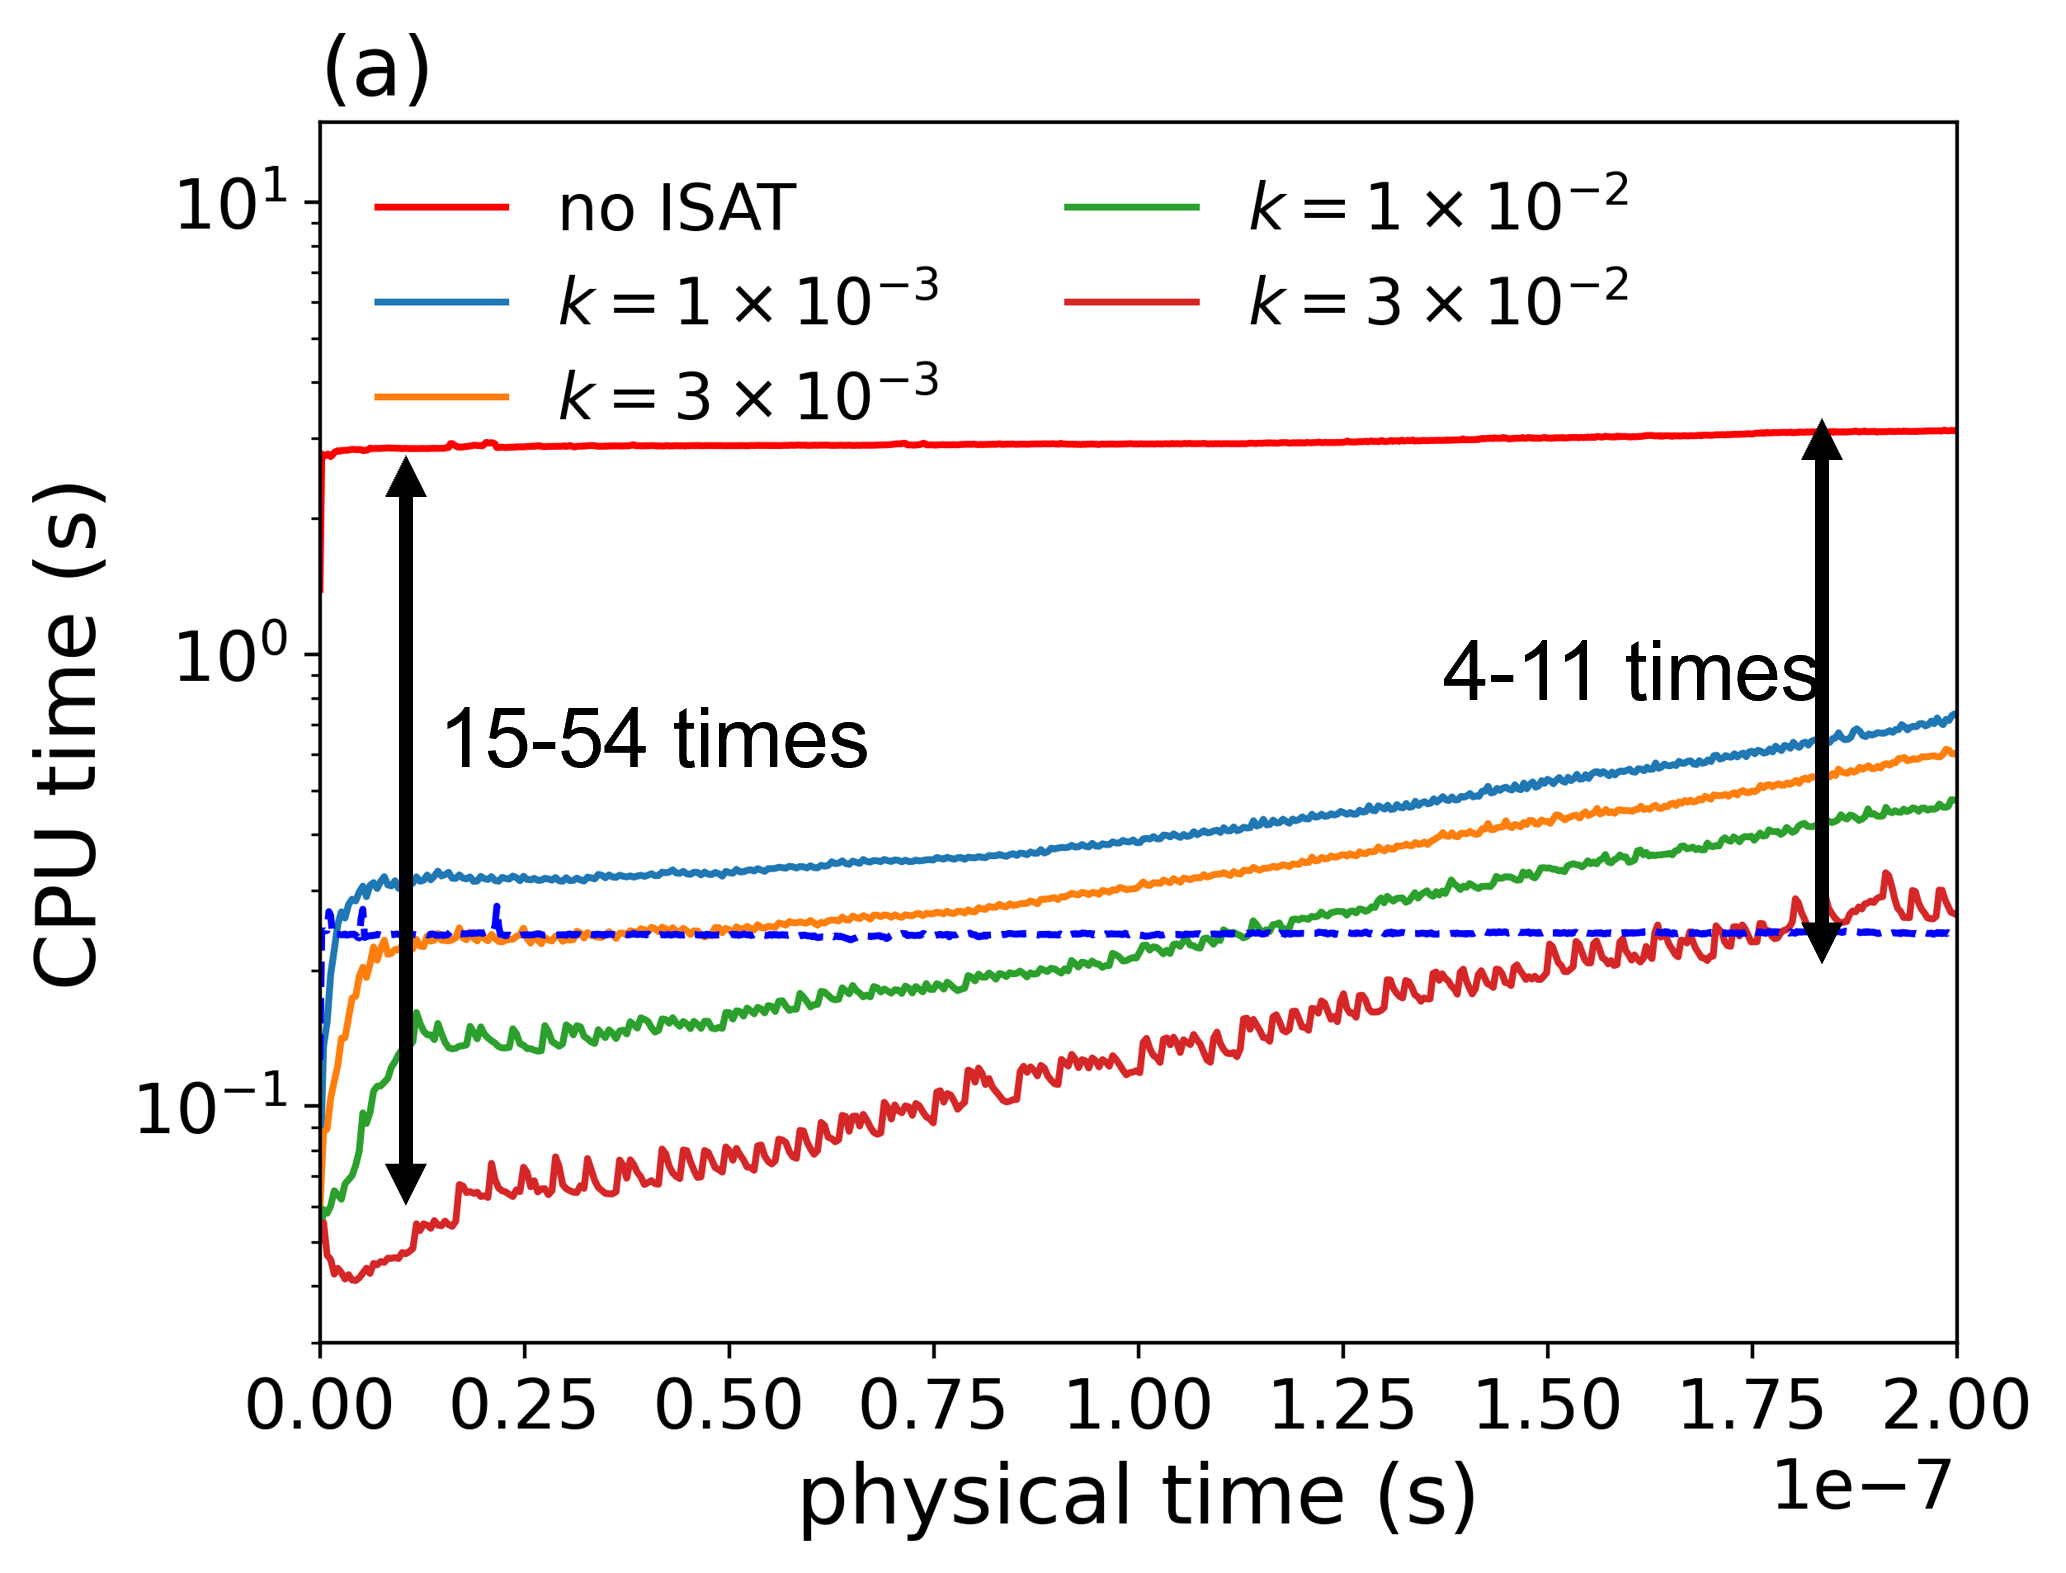
\includegraphics[width=0.45\linewidth]{time_TML_2D_m_2.png}
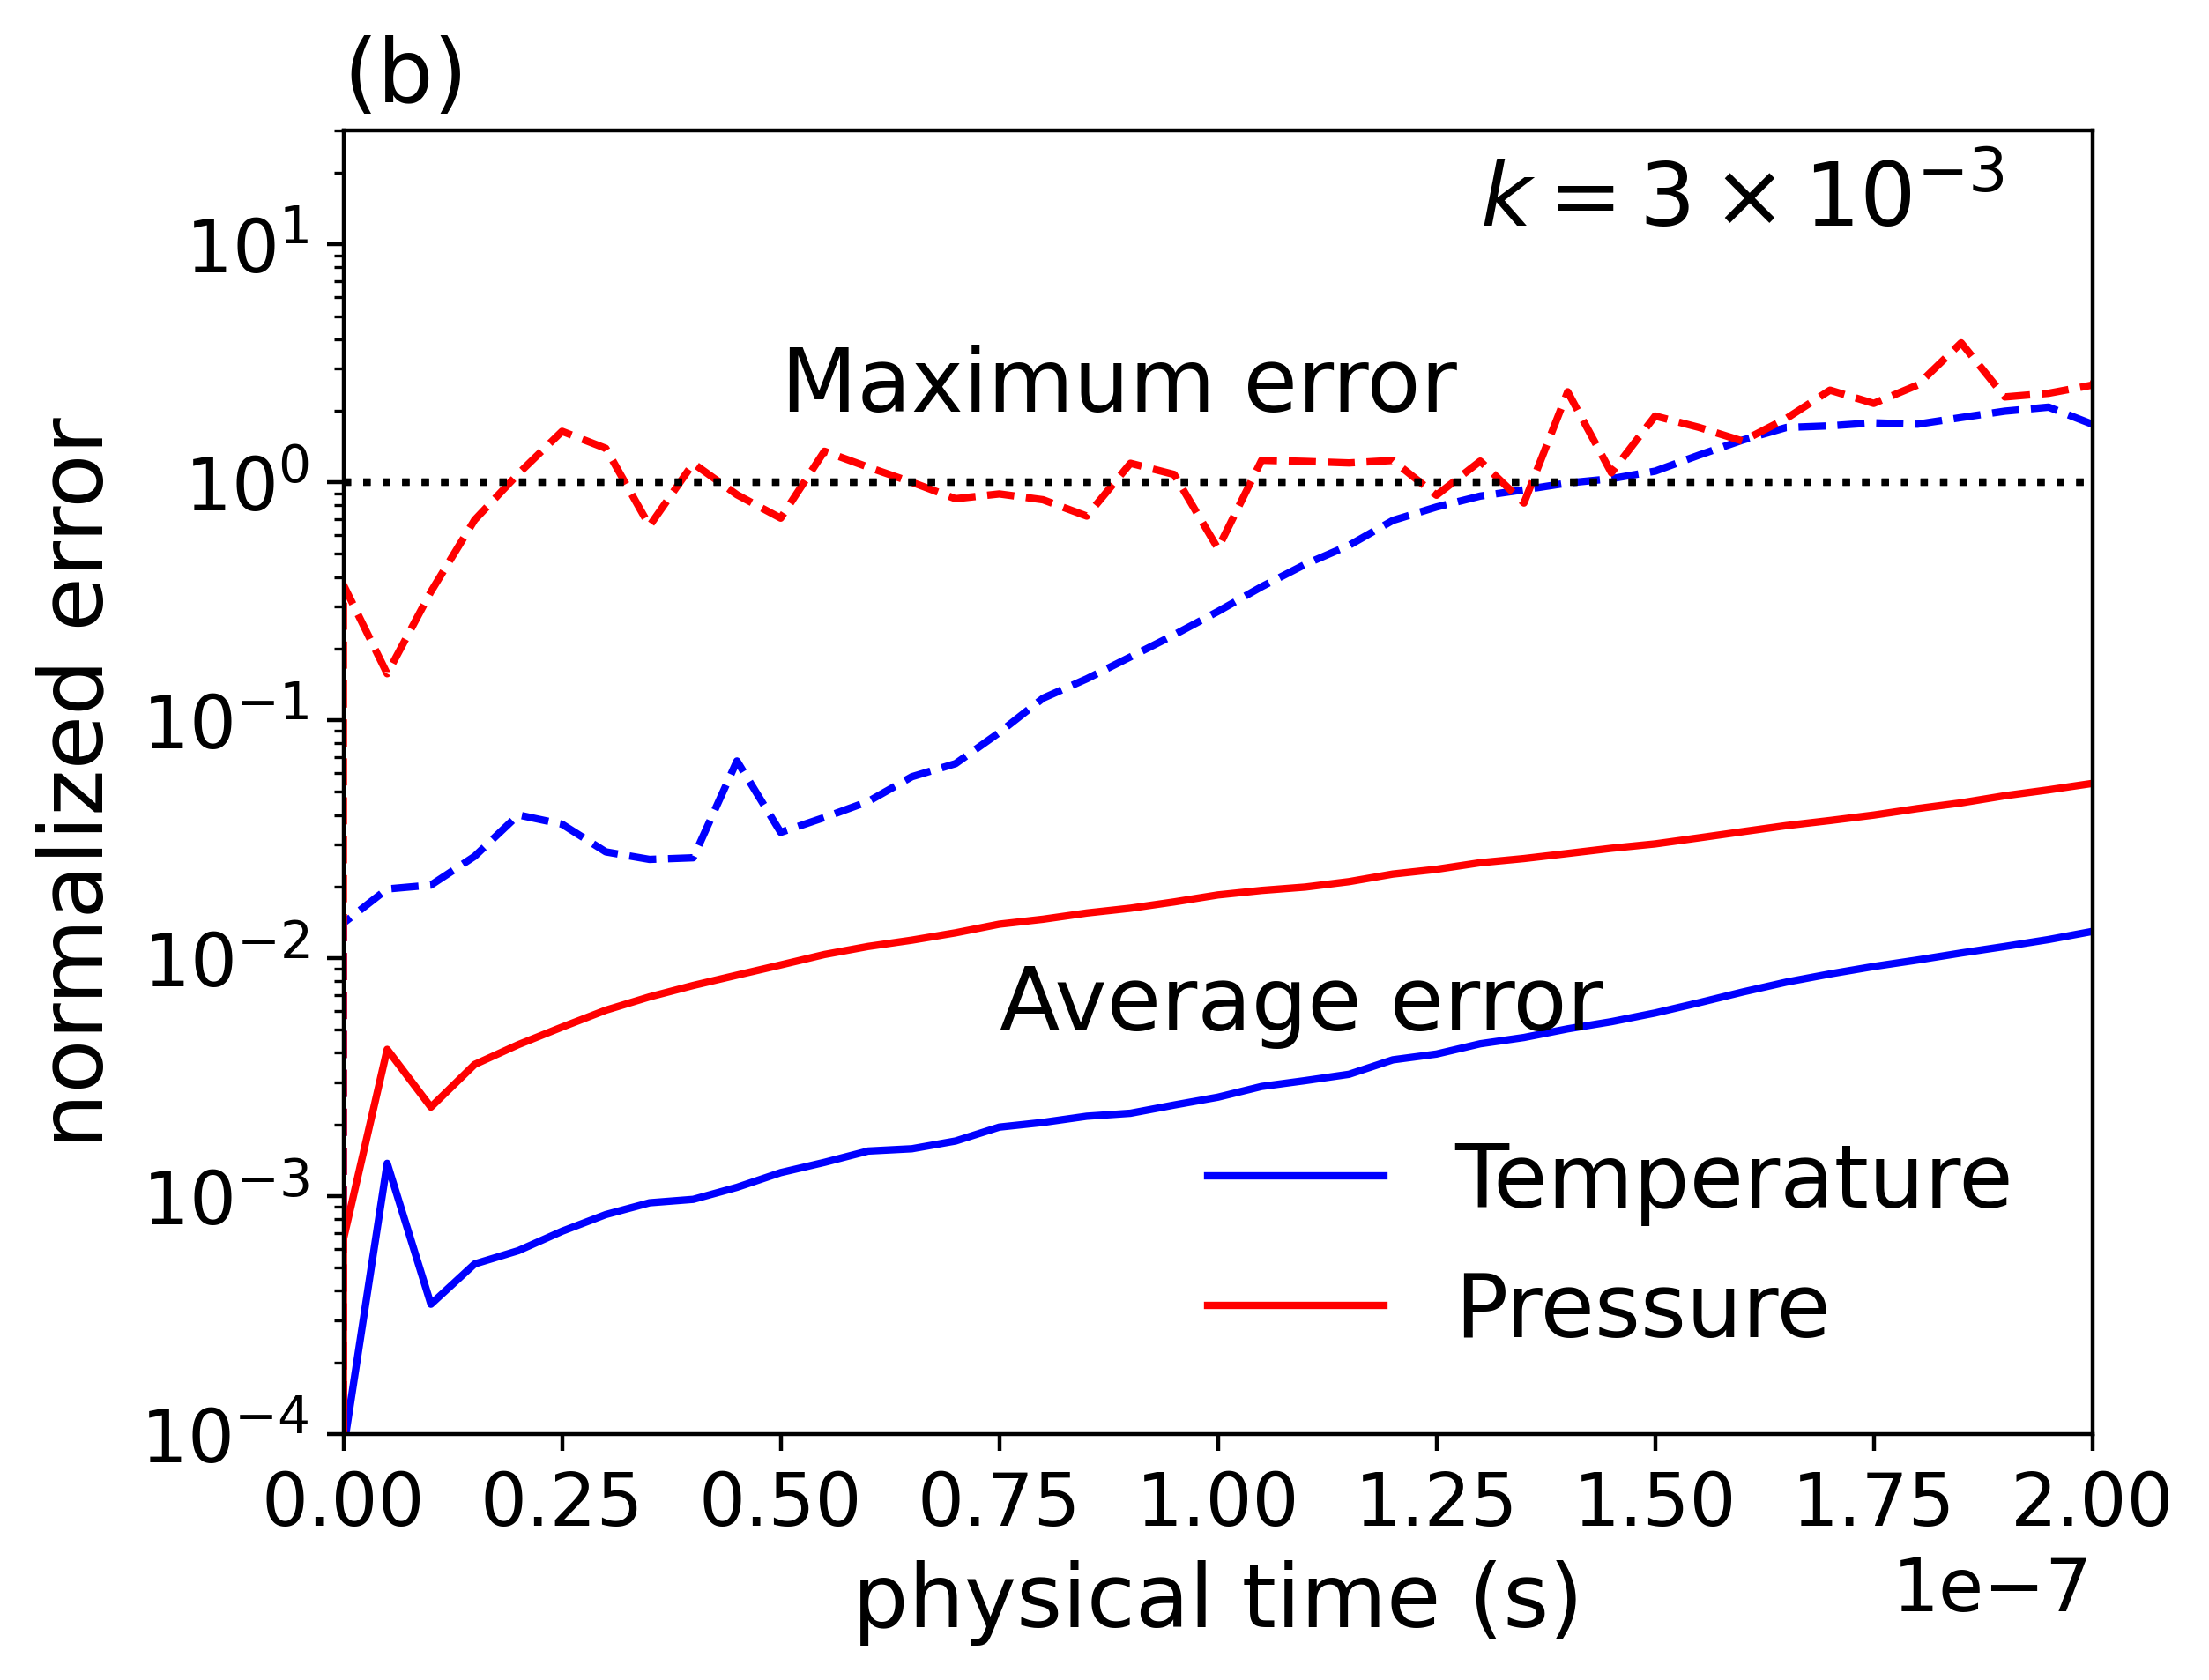
\includegraphics[width=0.45\linewidth]{error_TML_2D_3e_3_3.png}
\caption{(a) The performance of ISAT-VLE, in terms of the CPU time spent in every time step. The Blue dotted line is the CPU time of all other parts of the CFD solver, except the VLE model; the top red line is the CPU time of the VLE model without ISAT. In addition, 4 lines of the ISAT-VLE model with different tolerances ($k$) are provided. (b) The error control of ISAT-VLE, in terms of the normalized average error and maximum error versus physical time, $k=3\times 10^{-3}$.}
\label{TML_PE} 
\end{figure}




\begin{table}%[width=.9\linewidth,cols=4,pos=h]
\caption{The performance and errors of ISAT-VLE in TML cases with different error tolerance.}\label{TML_FC_table}
\begin{tabular*}{0.8\textwidth}{@{} l|lllll@{} }
\toprule
$k$                   & $1\times 10^{-3}$   & $3\times 10^{-3}$    & $1\times 10^{-2}$    &$3\times 10^{-2}$  \\%  & $1\times 10^{-1}$ \\
\midrule
Speed-up            & 6.7                  & 8.5                  & 11.6                 & 19.9                \\%  &  41.6          \\
$P$ mean error (bar) & $8.2\times 10^{-4}$  & $1.5\times 10^{-3}$  & $0.7\times 10^{-3}$  & $1.6\times 10^{-2}$\\%  & $2.8\times 10^{-1}$ \\
$P$ max error (bar)  & 0.06                 & 0.07                & 0.27                 & 1.0               \\% & 2.1              \\
$P$ max relative error (\%) &0.16                 & 0.20                & 0.71                 & 2.8           \\%     & 5.1              \\
$T$ mean error (K)   & $1.6\times 10^{-3}$  & $3.5\times 10^{-3}$  & $1.4\times 10^{-3}$  & $4\times 10^{-2}$ \\% & $7\times 10^{-1}$ \\
$T$ max error (K)    & 0.16                  & 0.6                  & 2.1                  & 6.4                \\%  &   60          \\
$T$ max relative error (\%) &0.05                 & 0.21                 & 0.73                 & 2.1             \\%   & 18.7              \\%
\bottomrule
\end{tabular*}
\end{table}

\subsection{Transcritical shock-droplet interaction}
\label{sec:SD}

In this section, transcritical shock-droplet interaction simulations are conducted to investigate the performance and error control of the ISAT-VLE method. The geometry of the initial setting is shown in Fig.~\ref{SD_GEO}, where $L=2$ mm and $l=0.5$ mm. A droplet of \ce{n-C12H26} with a diameter $d=0.25$ is positioned at the center of the domain, and the domain is filled with \ce{N2}. The initial pressure is set to 200 bar, and a high-pressure region of 800 bar is positioned on the left to generate a shock wave. The interfacial mass fraction of \ce{N2} is initialized using $\tanh(x/\omega)$, where $\omega=2 \times 10^{-6}$. The performance of ISAT-VLE is tested through both 2D and 3D simulations. In both cases, a uniform mesh size of $256\times256$ is utilized in the x-y plane. For the 3D simulations, the z direction consists of 256 uniformly spaced grid intervals. 


\begin{figure}[htbp]
\centering
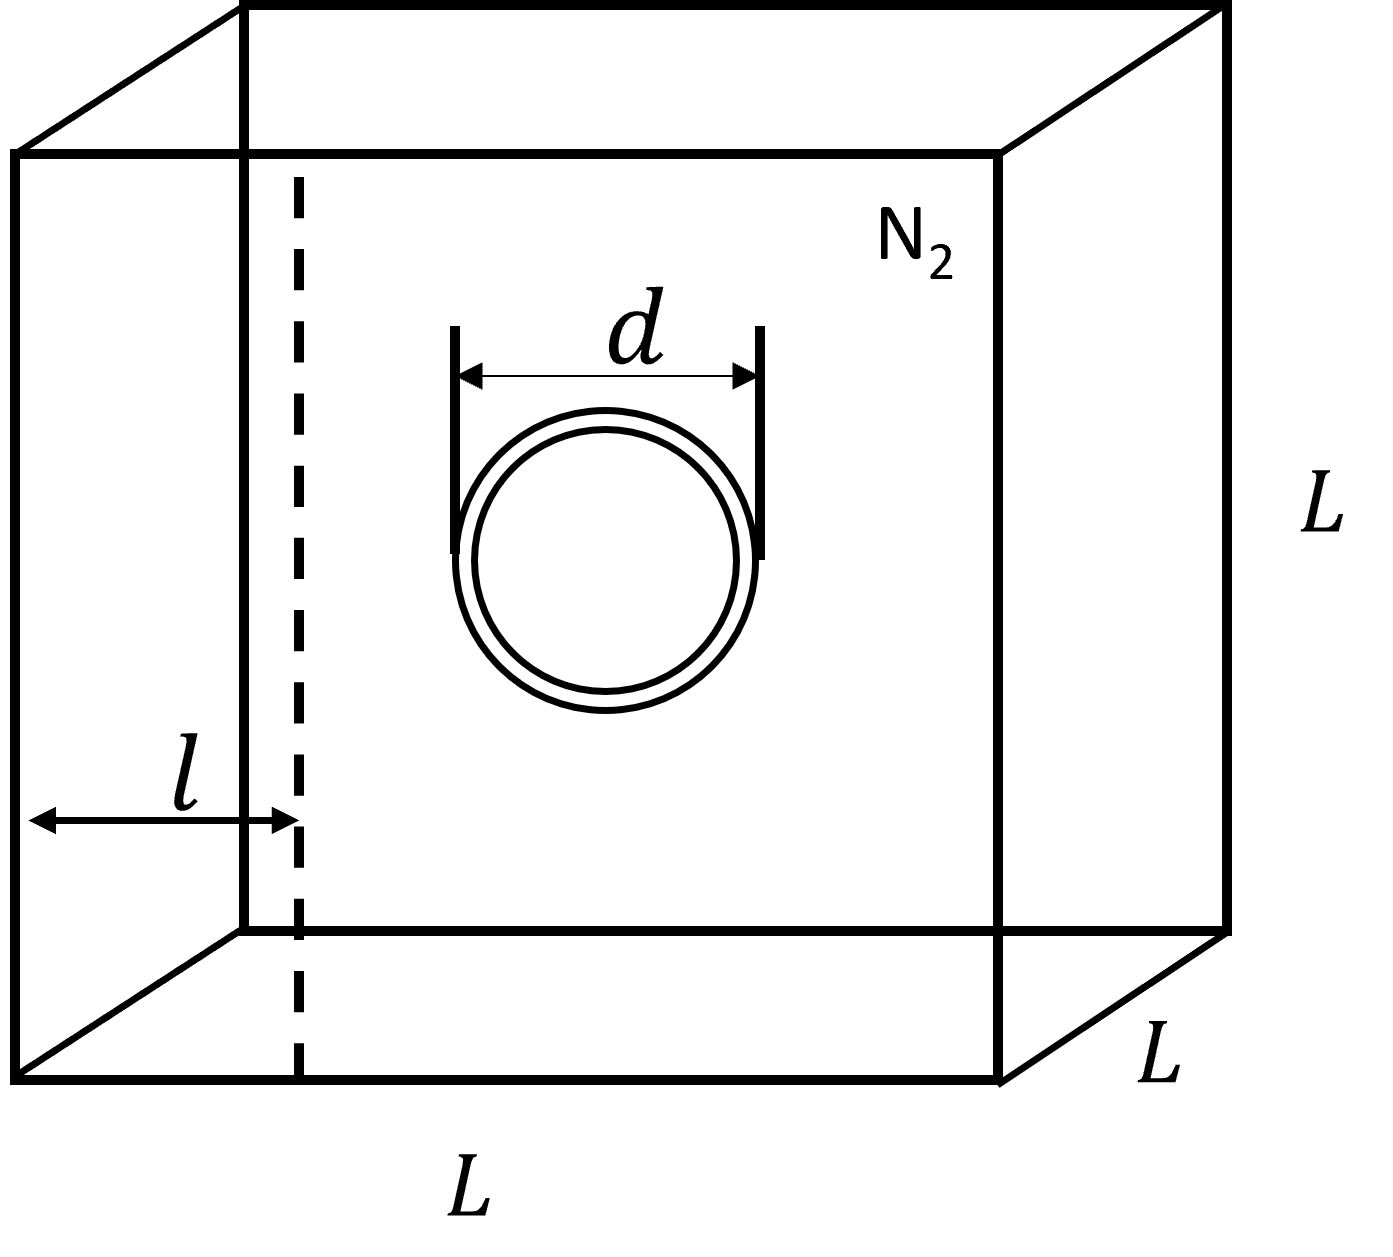
\includegraphics[width=0.35\linewidth]{ShockDrop_sc.png}
\hspace{.7in}
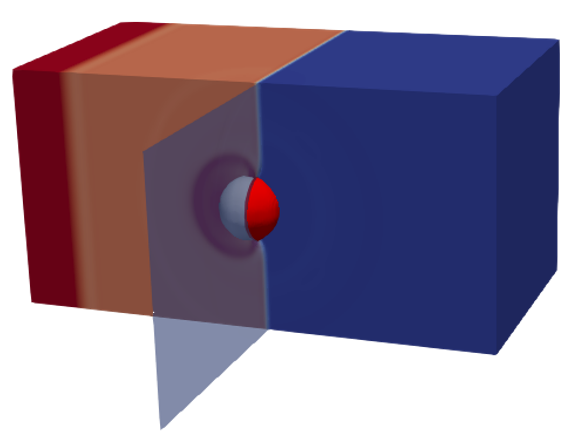
\includegraphics[width=0.30\linewidth]{2C_3d2.0080_s.png}
\caption{Left: geometry of the shock-droplet interaction simulations. The computational domain is of squared shape with side $L=2$mm. A high-pressure region with thickness $l=0.5$ mm is used to generate a shock wave. Droplet diameter: $d=0.25$ Right: pressure contours of the 3D shock-droplet interaction. Shock front: iso-surface of $P=30$ MPa; White color on the droplet surface: iso-surface of $Y_{C_{12}H_{26}}=0.7$; Red color on the droplet surface: iso-surface of $\beta =0.9$ to visualize the subcritical interface.}
\label{SD_GEO} 
\end{figure}

\subsubsection{ISAT-VLE's error control and tolerance in 2D simulations}
2D simulations are utilized to evaluate the error control of ISAT-VLE and select an appropriate error tolerance for later simulations. Throughout the entire computational domain, the initial temperature is set to 565 K, which is chosen specifically to examine the phase change effect in a multi-component droplet (refer to Sec.\ref{sec:SD_3D}). Initially, the fully conservative (FC) method results are presented. A range of error tolerance values are employed to assess performance, where the error tolerance $(T_{tol},p_{tol},\beta_{tol},c_{tol})$ is scaled by a factor $k$: specifically, the error tolerance values are set as $k (10^2, 10^7, 1, 10^2)$. The magnitude of these tolerances is based on the properties observed in these simulations. The error tolerance cases run until a physical time of $1\times 10^{-6}$s, at which point the shock wave has completely passed through the droplet. Fig.~\ref{droplet_PE}(a) illustrates the performance of ISAT-VLE. The top red line represents the CPU time cost of the VLE model without ISAT at each time step, while the blue dotted line corresponds to the CPU time cost of the remaining parts of the CFD solver. Both lines are insensitive to time. Compared with the rest part of the CFD solver, the VLE model without ISAT is computationally expensive, consistently utilizing around 90\% of the computational resources throughout this simulation. Prior to the interaction between the shock wave and the droplet, the computational costs of all ISAT-VLE cases with varying tolerances are similar. This is attributed to the simple thermodynamic states involved, where a limited data set in the ISAT-VLE table is sufficient to provide accurate approximations. Therefore, in this stage, the ISAT-VLE method exhibits excellent performance, with a speed-up factor of approximately 50, and the error tolerance has minimal impact on performance. As the shock-droplet interaction commences, the computational cost begins to increase, and the influence of the error tolerance becomes evident. Cases with larger tolerances demonstrate faster computation, and by a physical time of $1.5\times 10^{-6}$s, when the droplet has passed through the shock wave, the CPU times stabilize. At this stage, the case with the largest tolerance is approximately 22 times faster than the VLE model without ISAT, while even the slowest case is still around 11 times faster. 

The normalized ISAT error for the case with $k=3\times10^{-2}$ is depicted in Fig.~\ref{droplet_PE}(b). The error is normalized by its tolerance, and the dashed line represents an error equal to the normalized tolerance (error = 1), below which the error is controlled within the specified tolerance. The average error is three orders of magnitude smaller than the tolerance, and the maximum error is also within the tolerance. Table~\ref{droplet_FC_table} presents the errors and speed-up factors for all cases. Considering the initial pressure range (200 - 800 bar) and temperature (565 K) settings, the errors are acceptable, staying within 2\% for all different tolerances. For subsequent shock-droplet simulations, we choose $k=2 \times 10^{-3}$, which maintains the error within 1\% and provides sufficient accuracy.



\begin{figure}[htbp]
\centering
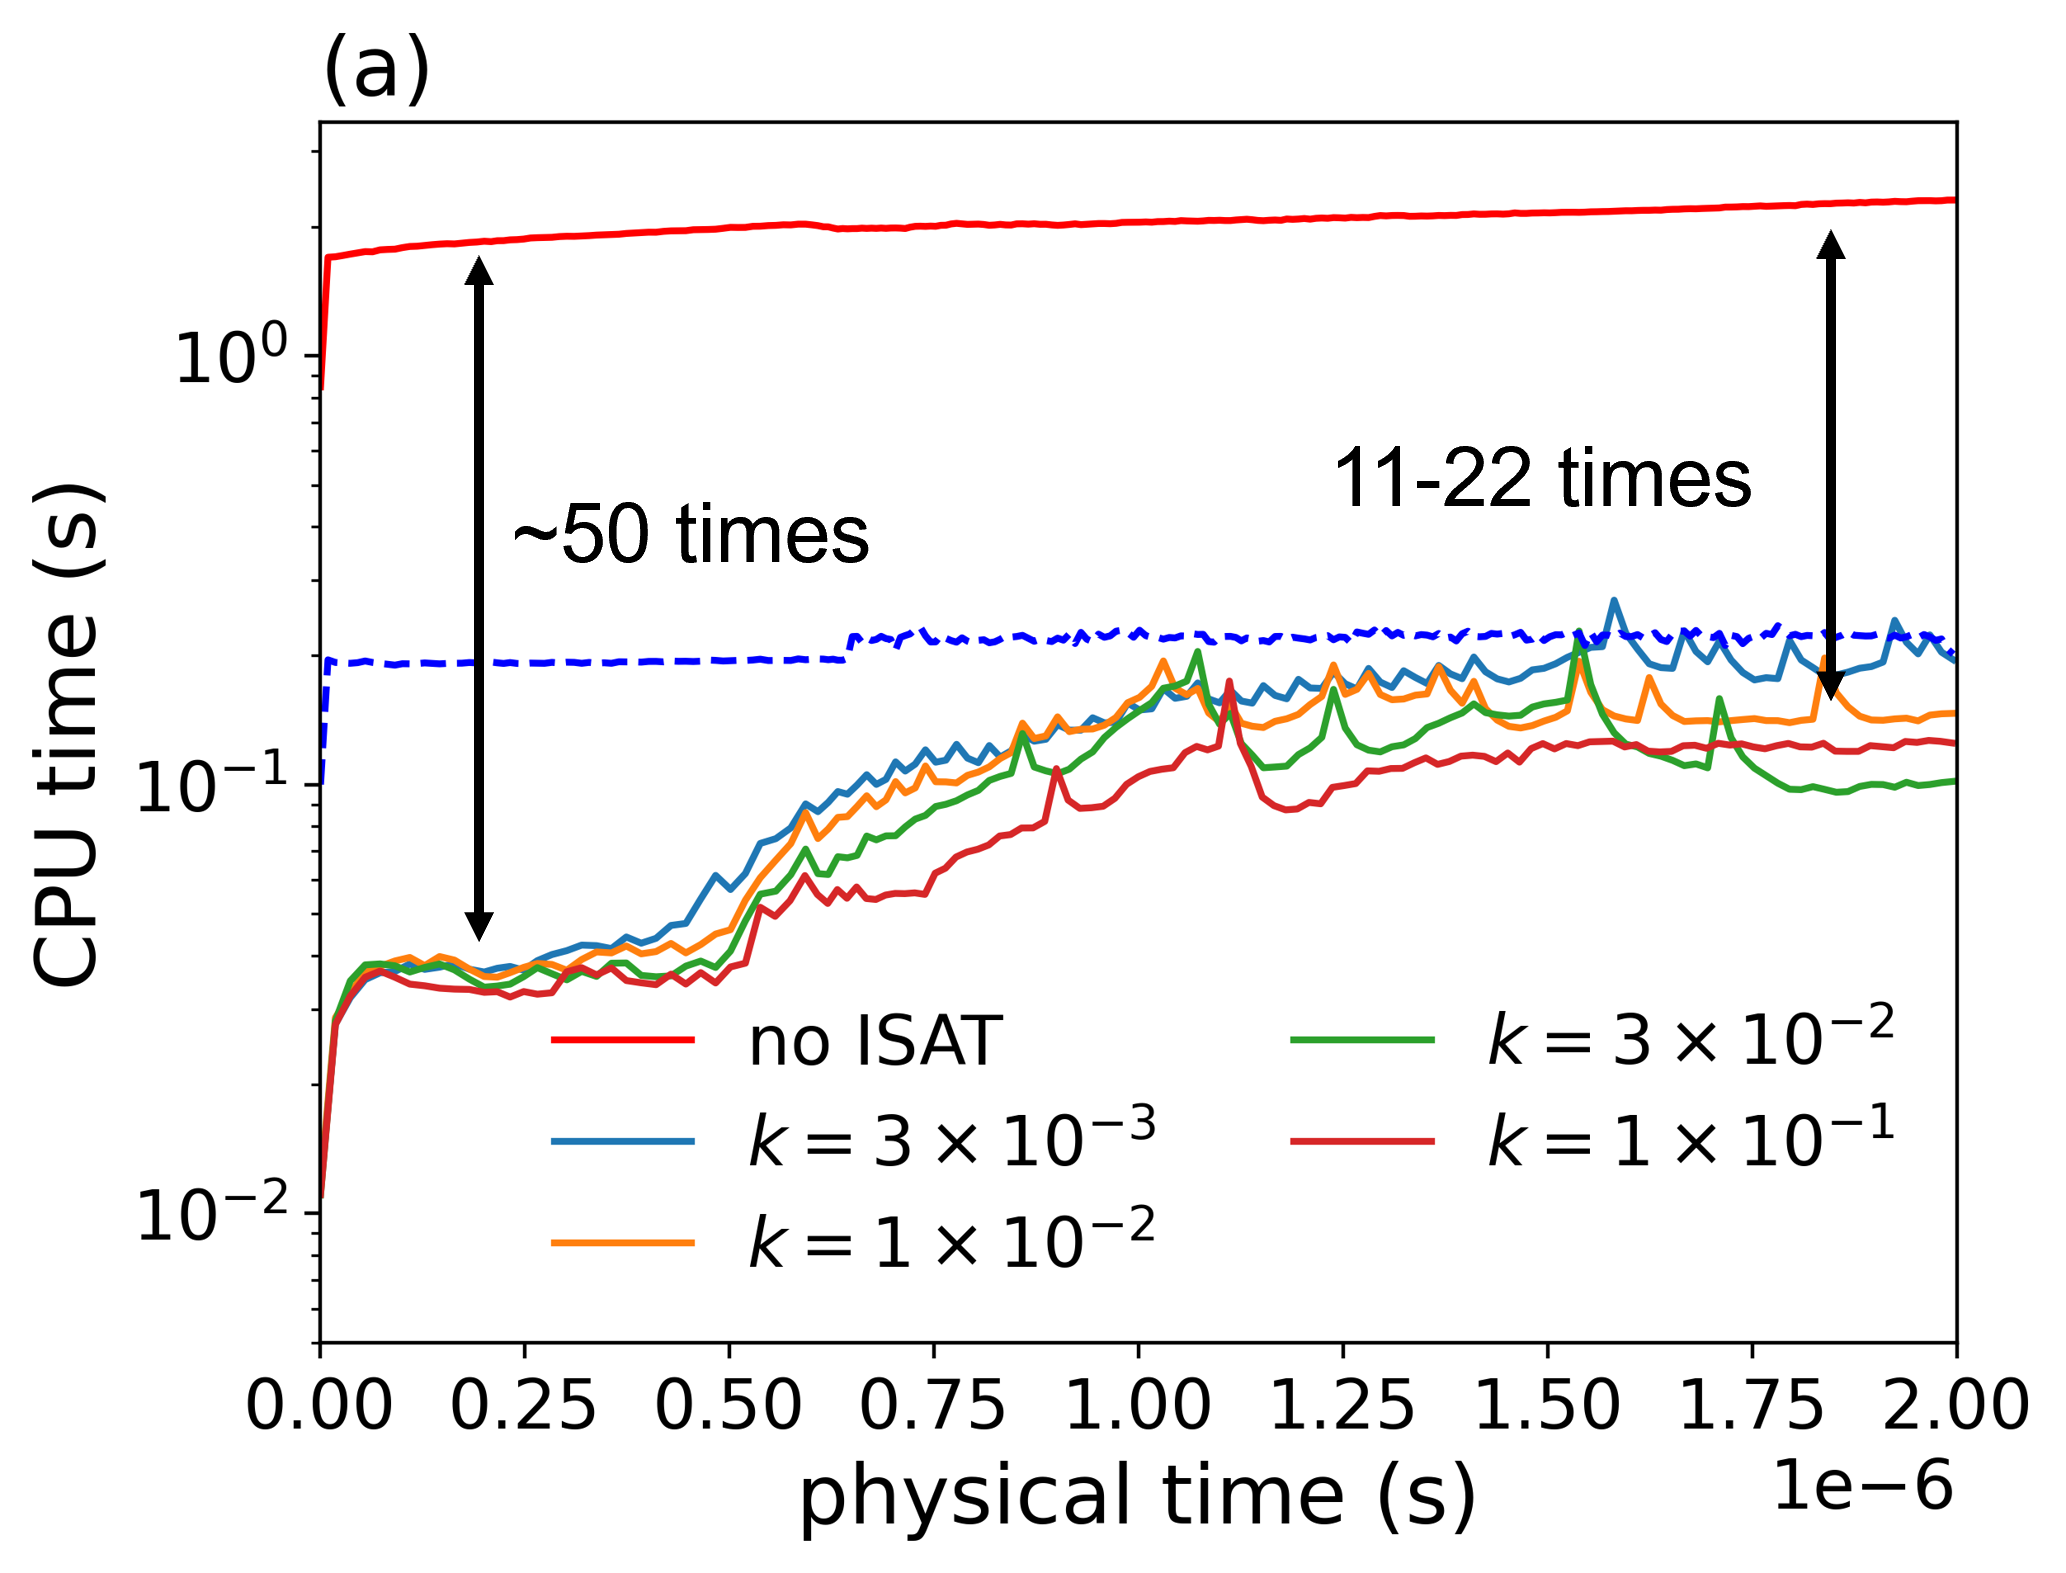
\includegraphics[width=0.45\linewidth]{time_droplet_C_2d_2_p.png}
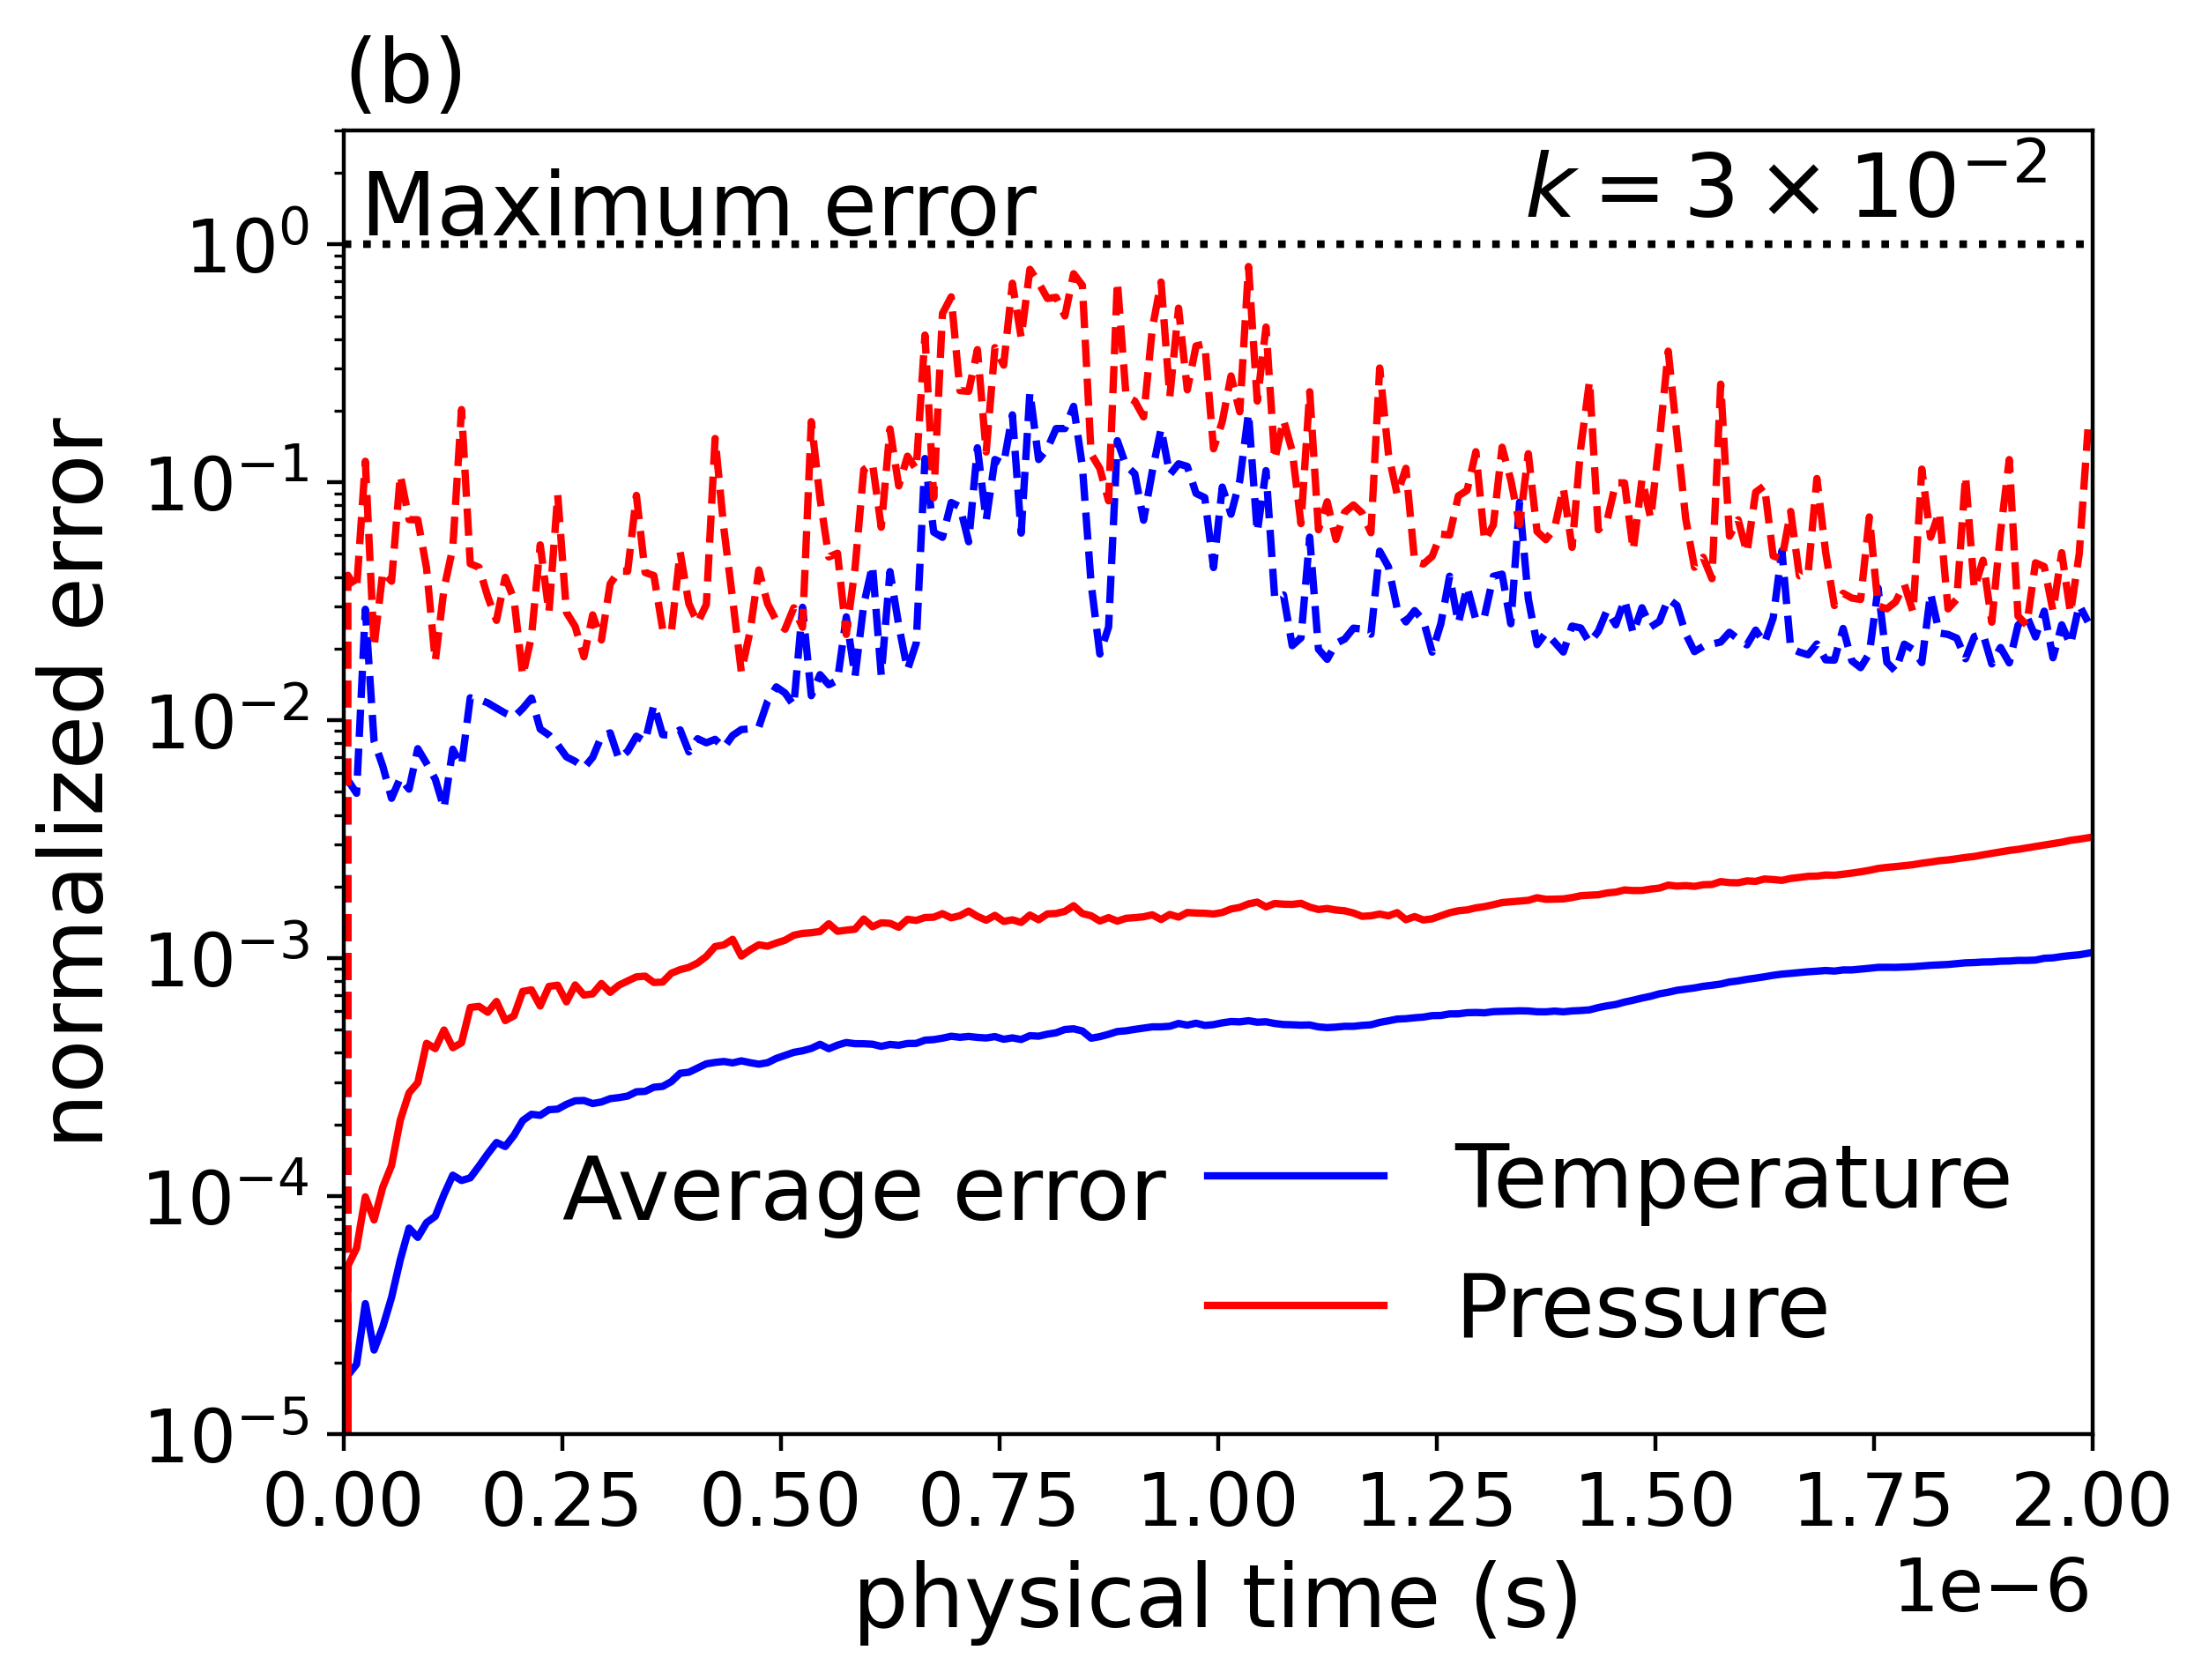
\includegraphics[width=0.45\linewidth]{error_droplet_C_2d.png}
\caption{(a) Performance of the ISAT-VLE method in the transcritical shock-droplet interaction simulation using the fully compressible (FC) scheme: the blue dotted line is the CPU time of all other parts of CFD solver, except the VLE model; the red line is the CPU time of VLE model without ISAT, and 4 lines of ISAT-VLE model with different tolerances ($k$) are provided. (b) The normalized error of the ISAT-VLE method with an error control of $k = 3 \times 10^{-2}$.}
\label{droplet_PE} 
\end{figure}



\begin{table}%[width=.9\linewidth,cols=4,pos=h]
\caption{The performance and error of the ISAT-VLE method in the transcritical shock-droplet interaction cases with different error tolerance.}\label{droplet_FC_table}
\begin{tabular*}{0.8\textwidth}{@{} l|lllll@{} }
\toprule
$k$                         & $3\times 10^{-3}$    & $1\times 10^{-2}$    &$3\times 10^{-2}$    & $1\times 10^{-1}$\\
\midrule
Speed-up                    & 15.3                 & 17.9                 & 20.9                &  23.8\\
$P$ mean error (bar)        & $2.4\times 10^{-4}$  & $1.8\times 10^{-3}$  & $9.6\times 10^{-3}$ & $8.8\times 10^{-2}$\\
$P$ max error (bar)         & 0.26                 & 0.86                 & 2.4                 & 7.7 \\
$P$ max relative error (\%) & 0.07                 & 0.2                  & 0.57                & 1.9 \\
$T$ mean error (K)          & $1.0\times 10^{-4}$  & $6.4\times 10^{-4}$  & $3.1\times 10^{-3}$ & $3.5\times 10^{-2}$\\
$T$ max error (K)           & 0.074                & 0.17                 & 0.71                & 2.2\\
$T$ max relative error (\%) & 0.012                & 0.029                & 0.12                & 0.36 \\
\bottomrule
\end{tabular*}
\end{table}

\subsubsection{Double flux scheme's behavior in 2D simulations}
\label{sec:DF}
We proceeded to perform a simulation using the double flux (DF) scheme to compare its behavior with the FC scheme. The ISAT-VLE error tolerance is set as $(T_{tol},e_{tol},\beta_{tol},c_{tol})= k (10^2, 10^4, 1, 10^2)$. Similar to the FC method,  performance improves when a larger tolerance is employed (Fig.~\ref{droplet_PE_D}(a)), but in comparison, the DF scheme runs even faster. Fig.~\ref{droplet_PE_D}(b) displays the normalized error (at $k=3 \times 10^{-2}$) It can be observed that the average error is controlled three orders of magnitude below the error tolerance. Although the maximum error cannot be entirely controlled within the tolerance due to the high non-linearity of the VLE system, the overall error remains within an acceptable range. The error and performance are listed in Tab.~\ref{droplet_DF_table}. When compared to the FC solver, the ISAT implementation in the DF solver achieves larger speedup factors ranging from 40 to 60, and exhibits significantly smaller pressure errors but slightly larger temperature errors. This discrepancy arises because, in the DF method, the pressure is directly obtained from the CFD solver, and its error is only influenced by the tabulation error of other properties, resulting in minimal pressure error. However, the DF scheme introduces stronger temperature oscillations (as depicted in Fig.~\ref{droplet_DC_compare} and discussed below), which contribute to an increased temperature error. Additionally, the double flux technique suppresses pressure oscillations, simplifying the thermal state and consequently leading to a larger speedup factor.



\begin{table}%[width=.9\linewidth,cols=4,pos=h]
\caption{The performance and error of the ISAT-VLE method using DF in the transcritical shock-droplet interaction cases with different error tolerance.}\label{droplet_DF_table}
\begin{tabular*}{0.8\textwidth}{@{} l|lllll@{} }
\toprule
$k$                        & $3\times 10^{-3}$   & $1\times 10^{-2}$    &$3\times 10^{-2}$    & $1\times 10^{-1}$\\
\midrule
Speed-up                   & 41.1                & 50.0                 & 60.9                & 63.9\\
$P$ mean error (bar)       & $6.7\times 10^{-5}$ & $2.2\times 10^{-4}$  & $2.4\times 10^{-4}$ & $1.2\times 10^{-3}$\\
$P$ max error (bar)        & $3.7\times 10^{-3}$ & $7.4\times 10^{-3}$  & $8.4\times 10^{-3}$ & $5.2\times 10^{-2}$ \\
$P$ max relative error (\%)& 0.001               & 0.002                & 0.003               & 0.016 \\
$T$ mean error (K)         & $3.9\times 10^{-3}$ & $1.1\times 10^{-3}$  & $2.8\times 10^{-3}$ & $7.5\times 10^{-3}$\\
$T$ max error (K)          & 0.14                & 4.43                 & 4.52                & 9.39\\
$T$ max relative error (\%)& 0.02                & 0.76                 & 0.78                & 1.5 \\
\bottomrule 
\end{tabular*}
\end{table}

\begin{figure}[htbp]
\centering
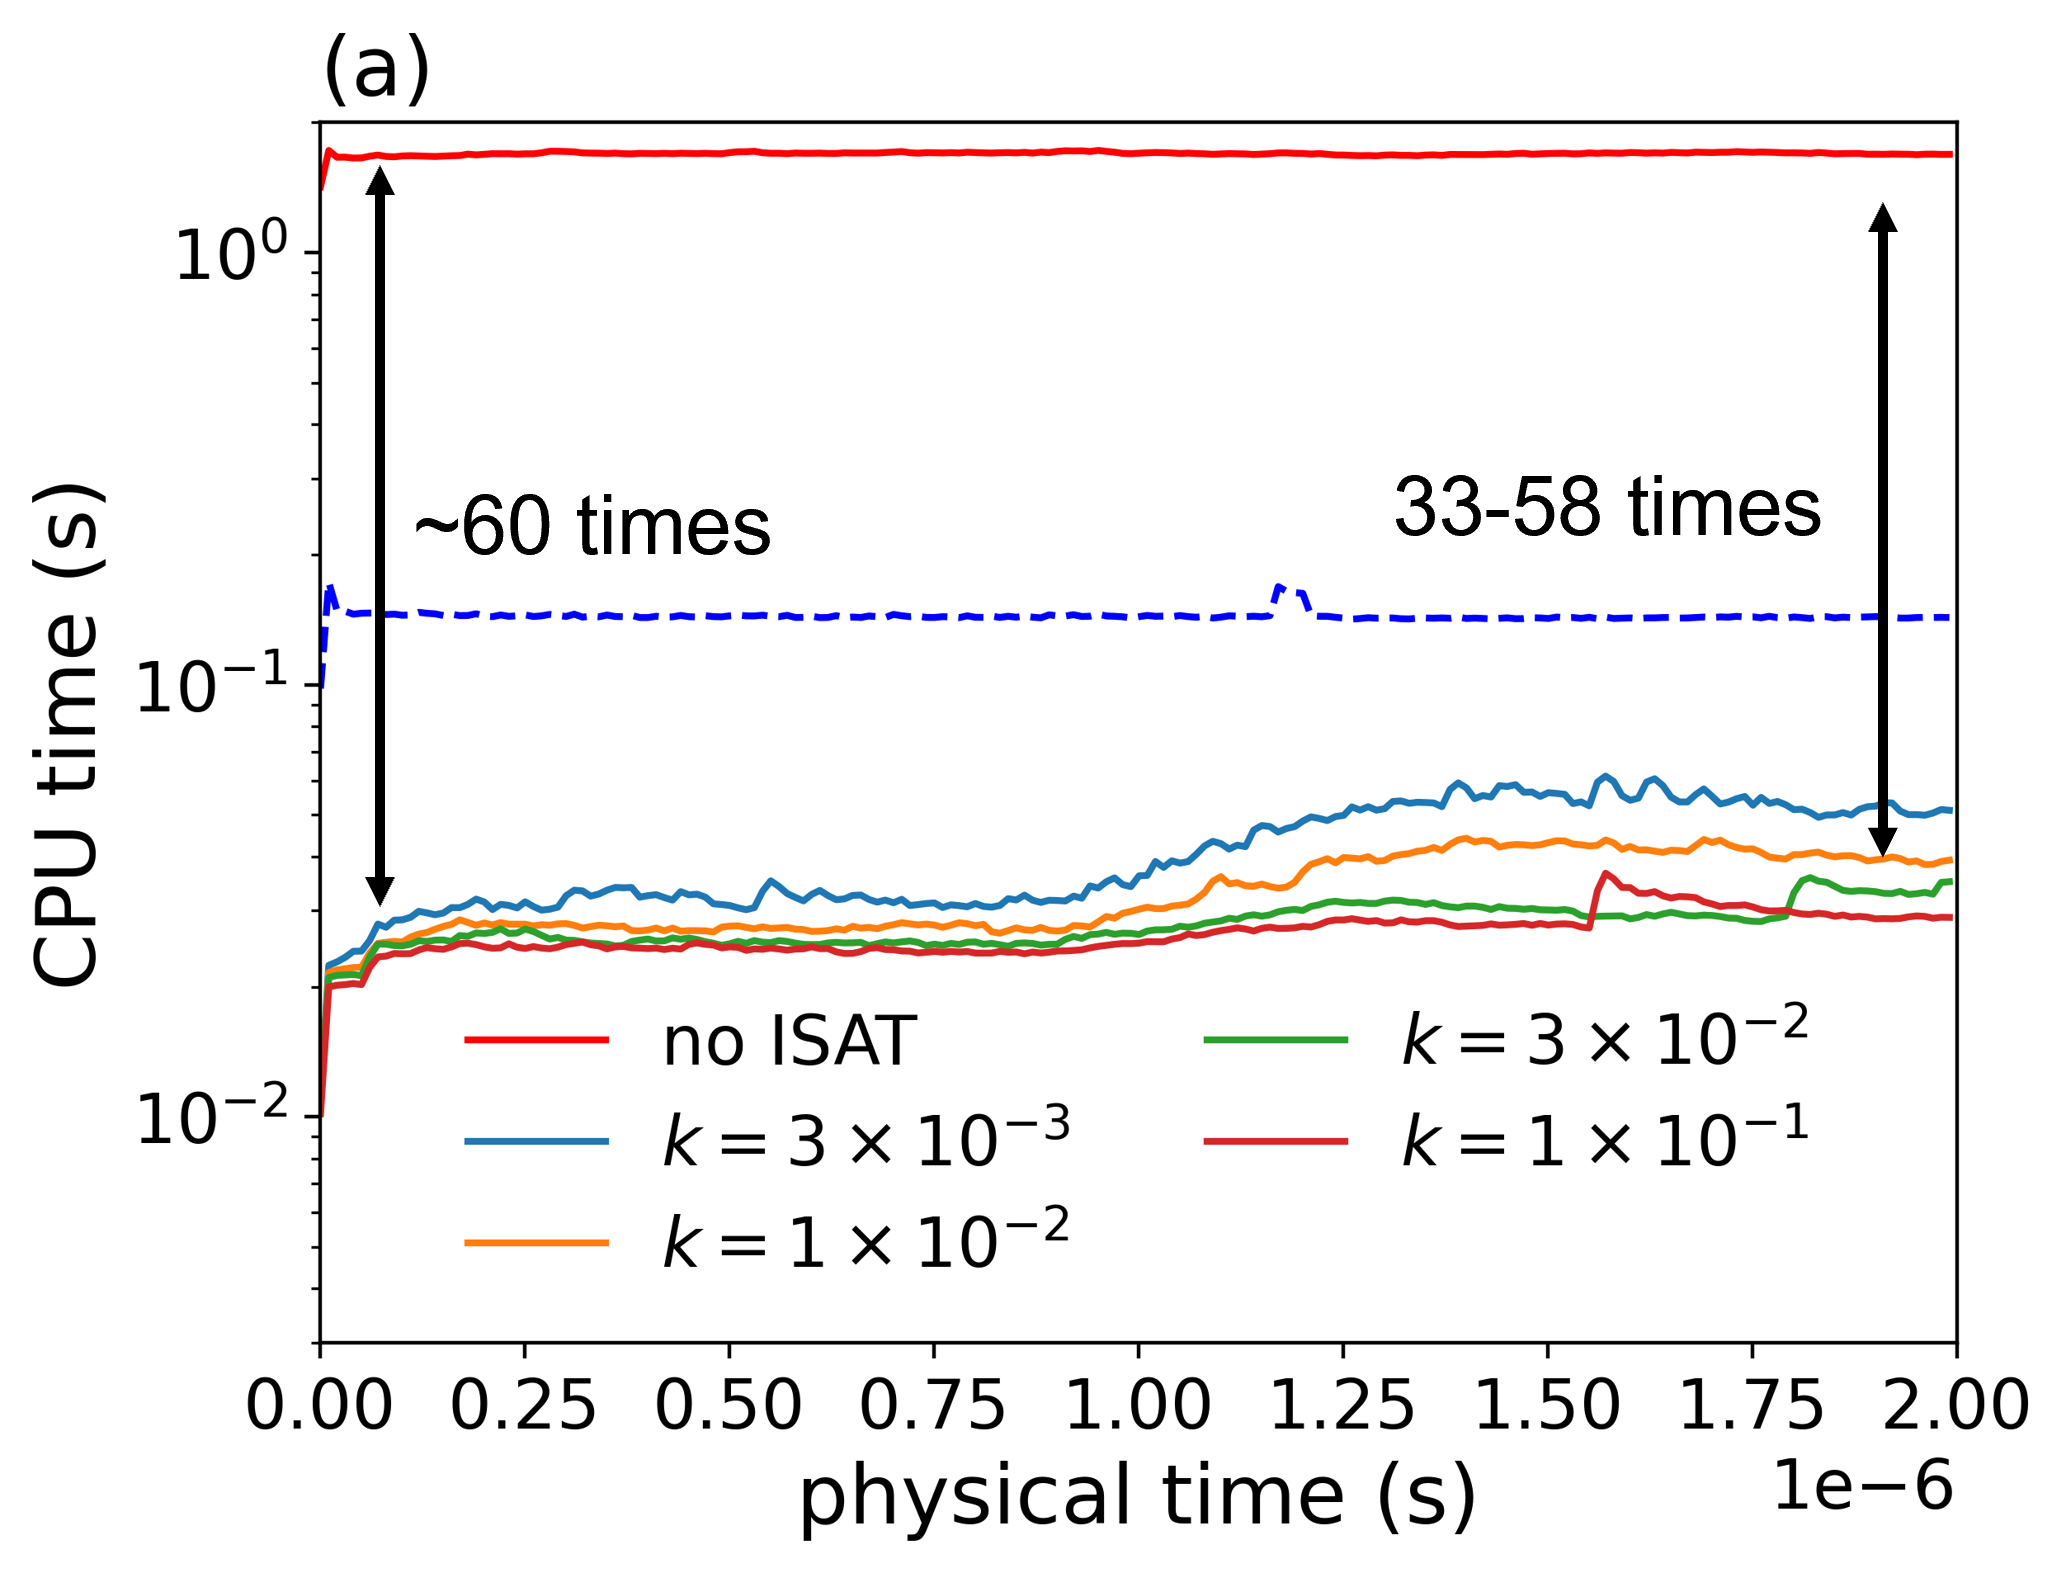
\includegraphics[width=0.45\linewidth]{time_droplet_D_2d_2_p.png}
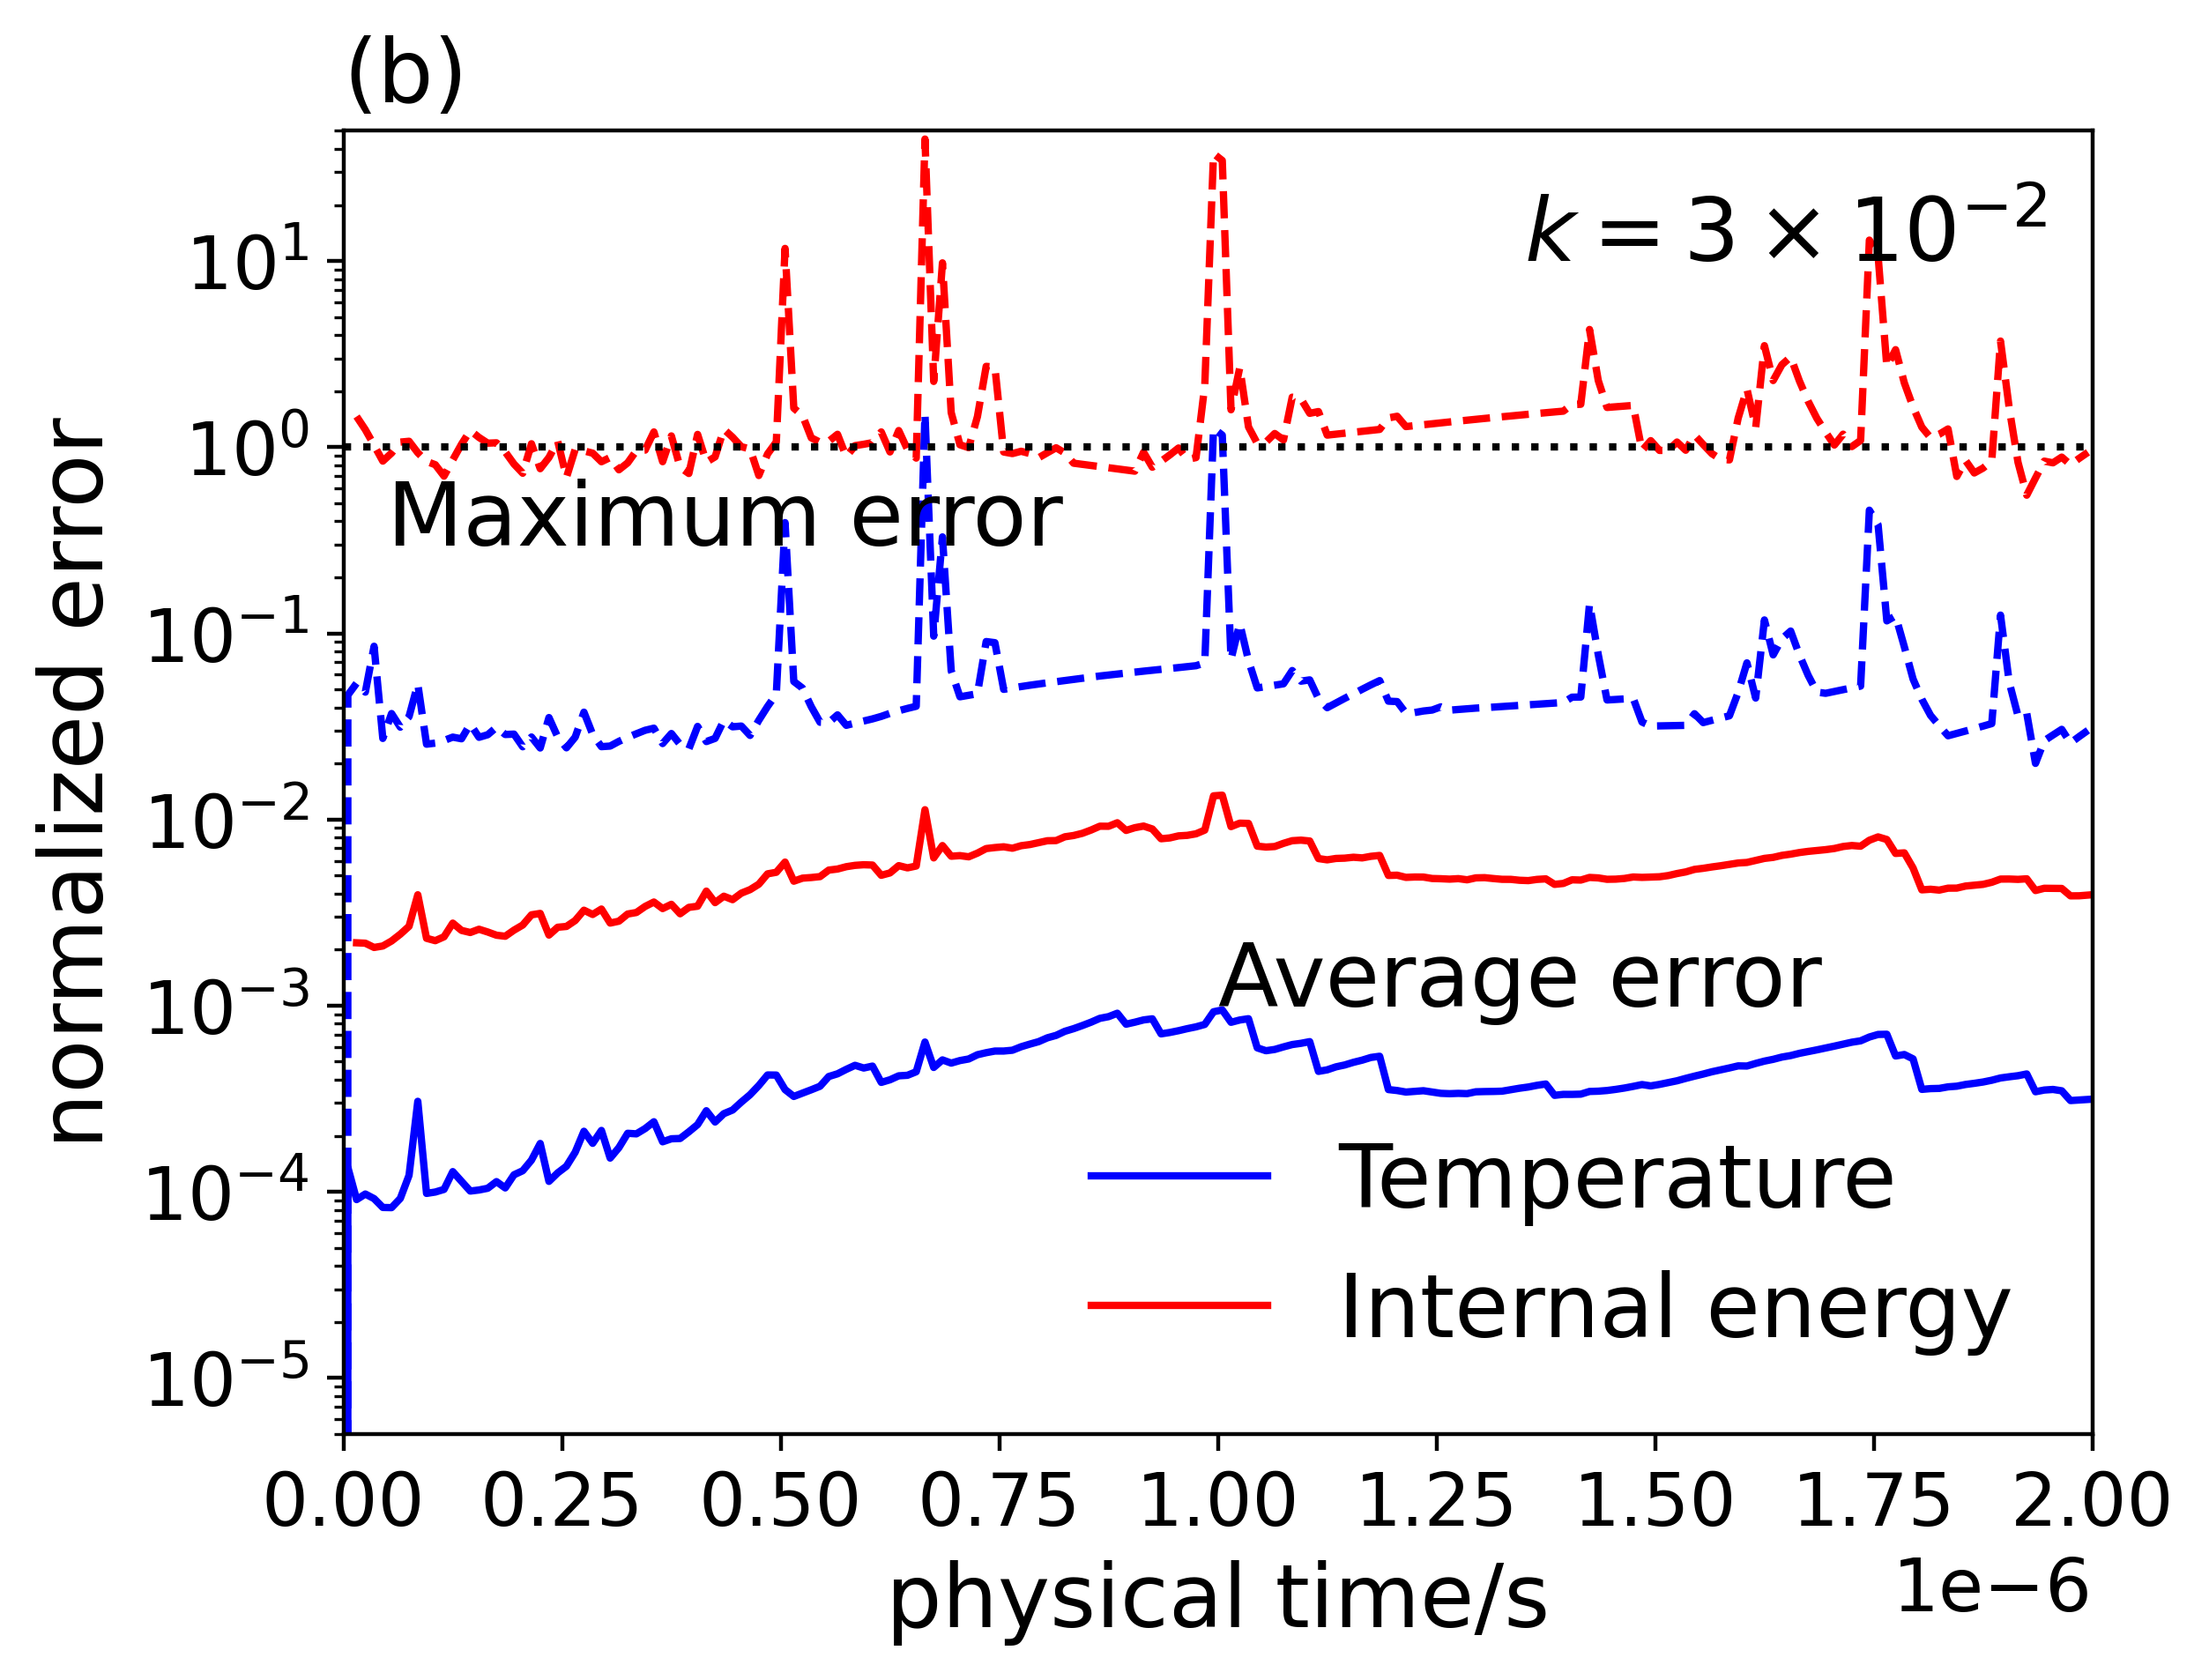
\includegraphics[width=0.45\linewidth]{error_droplet_D_2d_2.png}
\caption{(a) Performance of the ISAT-VLE method in the transcritical shock-droplet interaction simulation using the double flux (DF) scheme: the blue dotted line is the CPU time of all other parts of CFD solver, except the VLE model; the red line is the CPU time of VLE model without ISAT, and 4 lines of ISAT-VLE model with different tolerances ($k$) are provided. (b) The normalized error of the ISAT-VLE method with an error control of $k = 3 \times 10^{-2}$.}
\label{droplet_PE_D} 
\end{figure}

To mitigate the spurious oscillation resulting from real fluid effects, quasi-conservative methods are commonly employed to suppress or eliminate these oscillations. One popular approach among them is the DF method. However, it is important to note that these methods come at the cost of breaking the energy conservation law. In Fig.~\ref{droplet_DC_compare}, a comparison is made between the DF and the FC results in terms of pressure and temperature along the centerline in the x direction. This comparison is conducted when the shock wave has not yet reached the droplet position, allowing for separate analysis of the effects of the two methods on the shock wave and droplet. Without the DF method, the real fluid effect generates pressure and temperature oscillations at the droplet interface. On the other hand, the DF method successfully eliminates pressure oscillations at the droplet interface, which is the intended goal of this scheme's design. However, in order to achieve this, energy is added/removed to the discontinuity, resulting in larger temperature oscillations at the droplet interface. Additionally, breaking the energy conservation law introduces larger oscillations at the shock wave front. While some researchers argue that the energy introduced by the DF method decreases as the mesh is refined, it is often impractical to use a fine enough mesh to solve the droplet interface for 2D or 3D simulations. Therefore, breaking the energy conservation law is not considered an optimal solution. 

When the pressure oscillation in the simulation is substantial enough to cause the solution to diverge, it is preferable to allow for larger temperature oscillations while eliminating pressure oscillations. On the other hand, in simulations where temperature does not play a crucial role, the DF scheme can also be a suitable option. Conversely, when the simulation results are highly sensitive to temperature, the FC scheme is a better choice. This is precisely why we predominantly utilize the FC methods in our simulations, as the VLE process is particularly sensitive to temperature at the interface.



\begin{figure}[htbp]
\centering
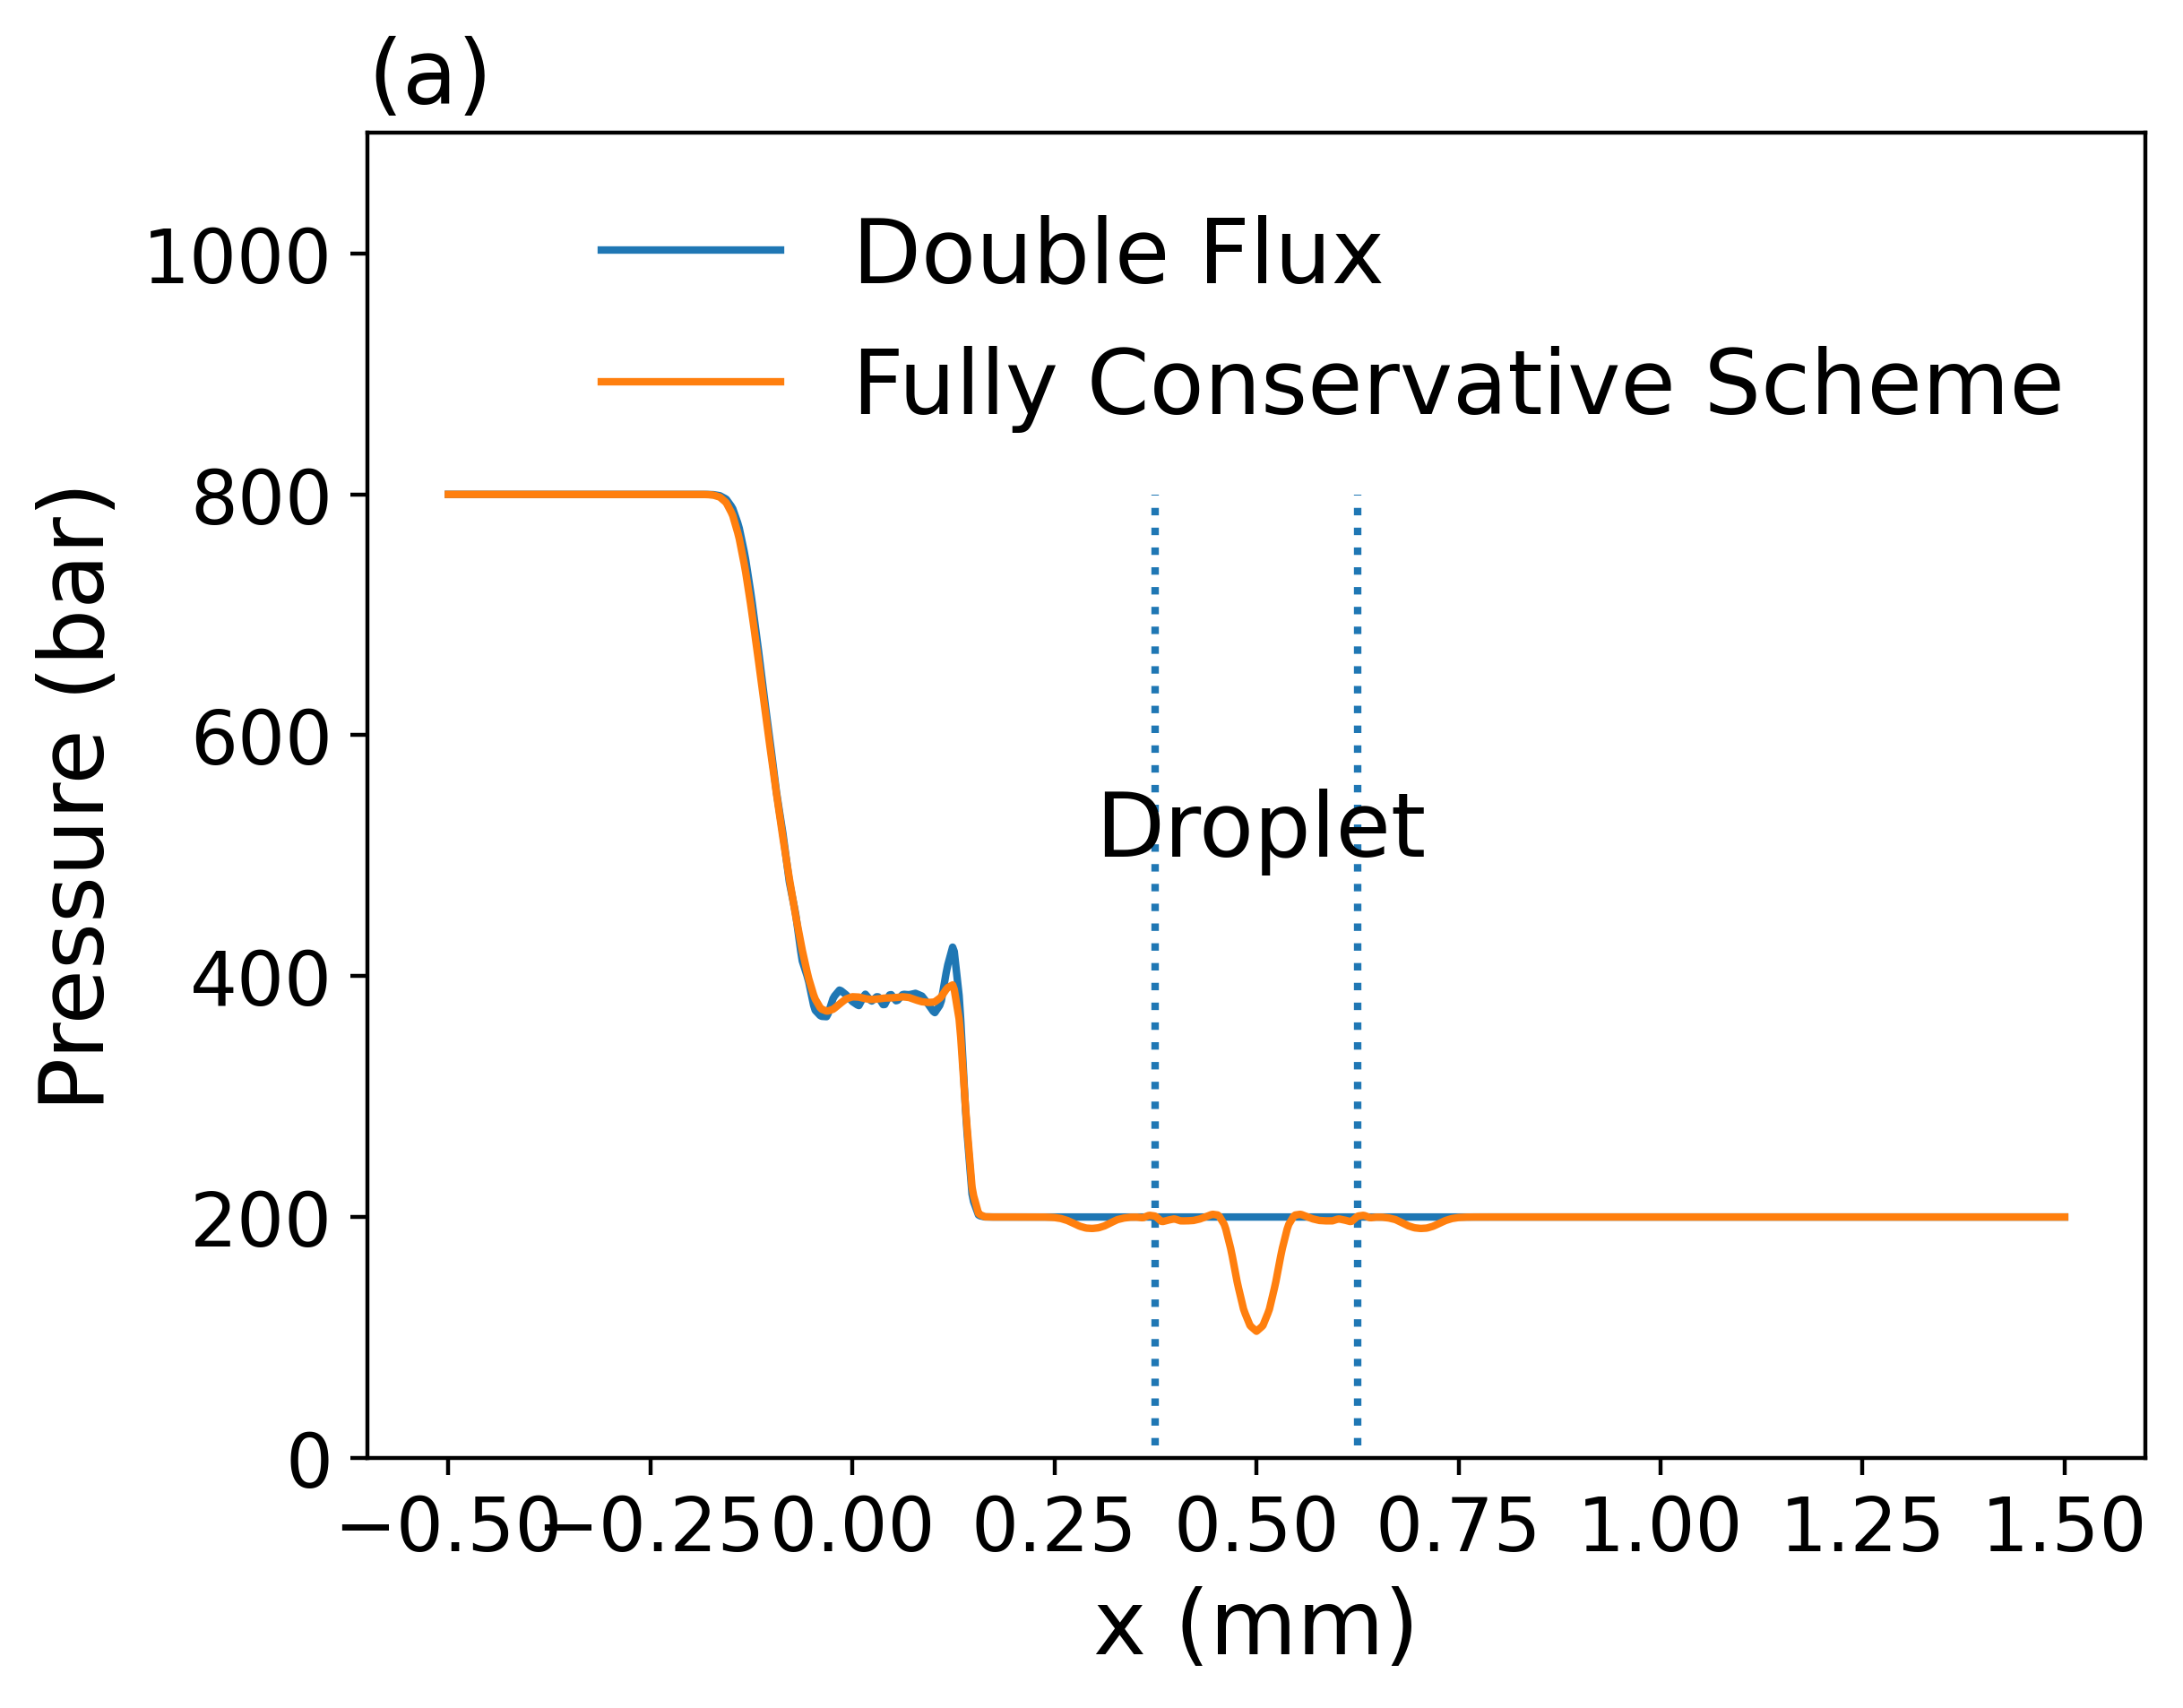
\includegraphics[width=0.4\linewidth]{DC_compare_2e_7_p.png}
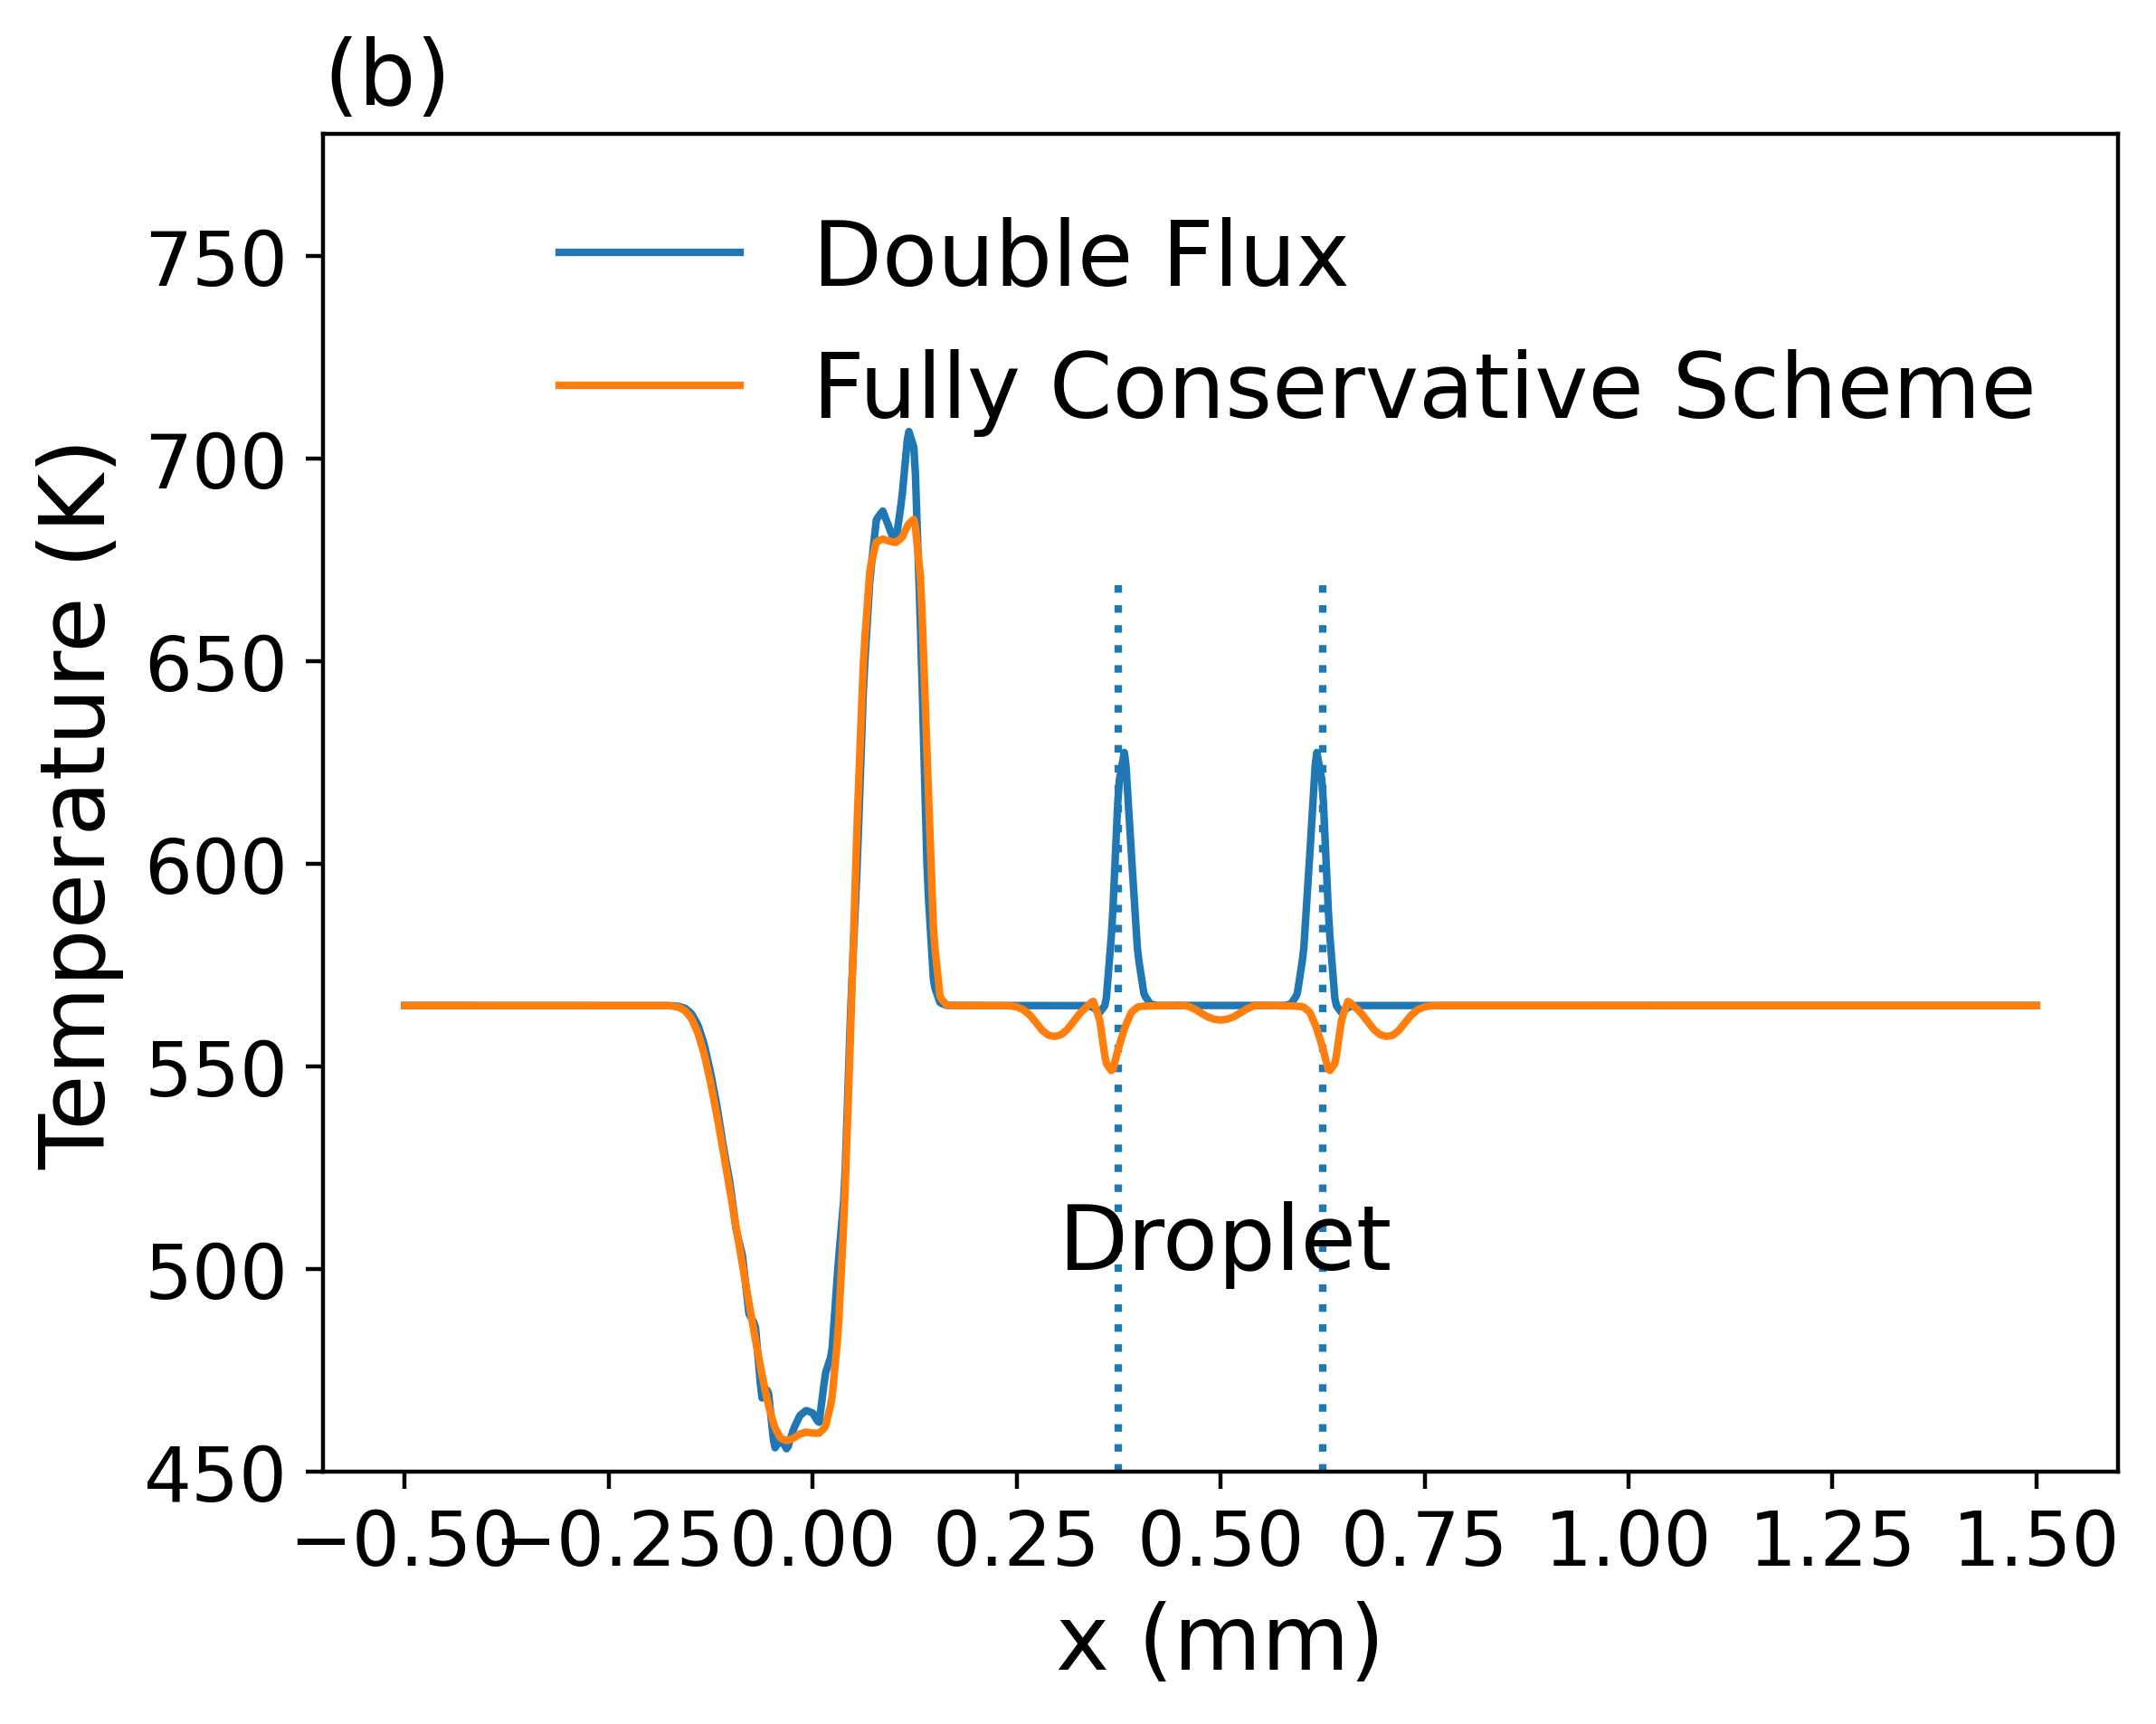
\includegraphics[width=0.4\linewidth]{DC_compare_2e_7_T.png}
\caption{Comparison between fully conservative (FC) scheme and double flux (DF) method results: (a) pressure, and (b) temperature. The results show the properties at the horizontal center line along $x$ direction through the droplet center.}
\label{droplet_DC_compare} 
\end{figure}

\subsubsection{Redundant records deletion methods}
\label{sec:delete}
In Sec.\ref{sec:ISAT}, we introduced new methods for deleting redundant records, and in this subsection, we assess their performance through shock-droplet interaction simulations using the FC scheme. Sec.\ref{sec:ISAT} illustrates the test results. First, we examined the outcomes without active data removal (FS: fixed maximum table size). Three different maximum table sizes were employed (FS1: 140,000, FS2: 130,000, FS3: 120,000). It can be observed that the FS3 result is slower compared to FS1 and FS2. This is because the maximum table size in FS3 is insufficient to store an adequate number of records , leading to more VLE problem-solving and thus reducing performance. Once the table size is adequately large, further increasing the maximum size no longer significantly impacts performance. Hence, the results for FS1 and FS2 are close to the limits of this method.

Next, we conducted separate tests for our proposed methods: the maximum unused step method (MUS) and the adaptive maximum table size method (AS). In MUS, we actively eliminate data that hasn't been used within the last 80 time steps. In AS, we utilized parameters $C = 5.8$ and $M = 5$ to update the maximum table size (Eq.\ref{eq:adap}). Both methods resulted in reduced CPU time and achieved approximately a 4\% performance improvement. When both methods were used concurrently (AS+MUS), the performance was further enhanced by approximately 2\%. It is worth noting that the ISAT method has already undergone substantial optimization, effectively utilizing computational resources. However, we identified additional optimization opportunities, and our methods still yielded a 6\% performance improvement. This AS+MUS method was employed for all simulations in this study.


\begin{figure}[htbp]
\centering
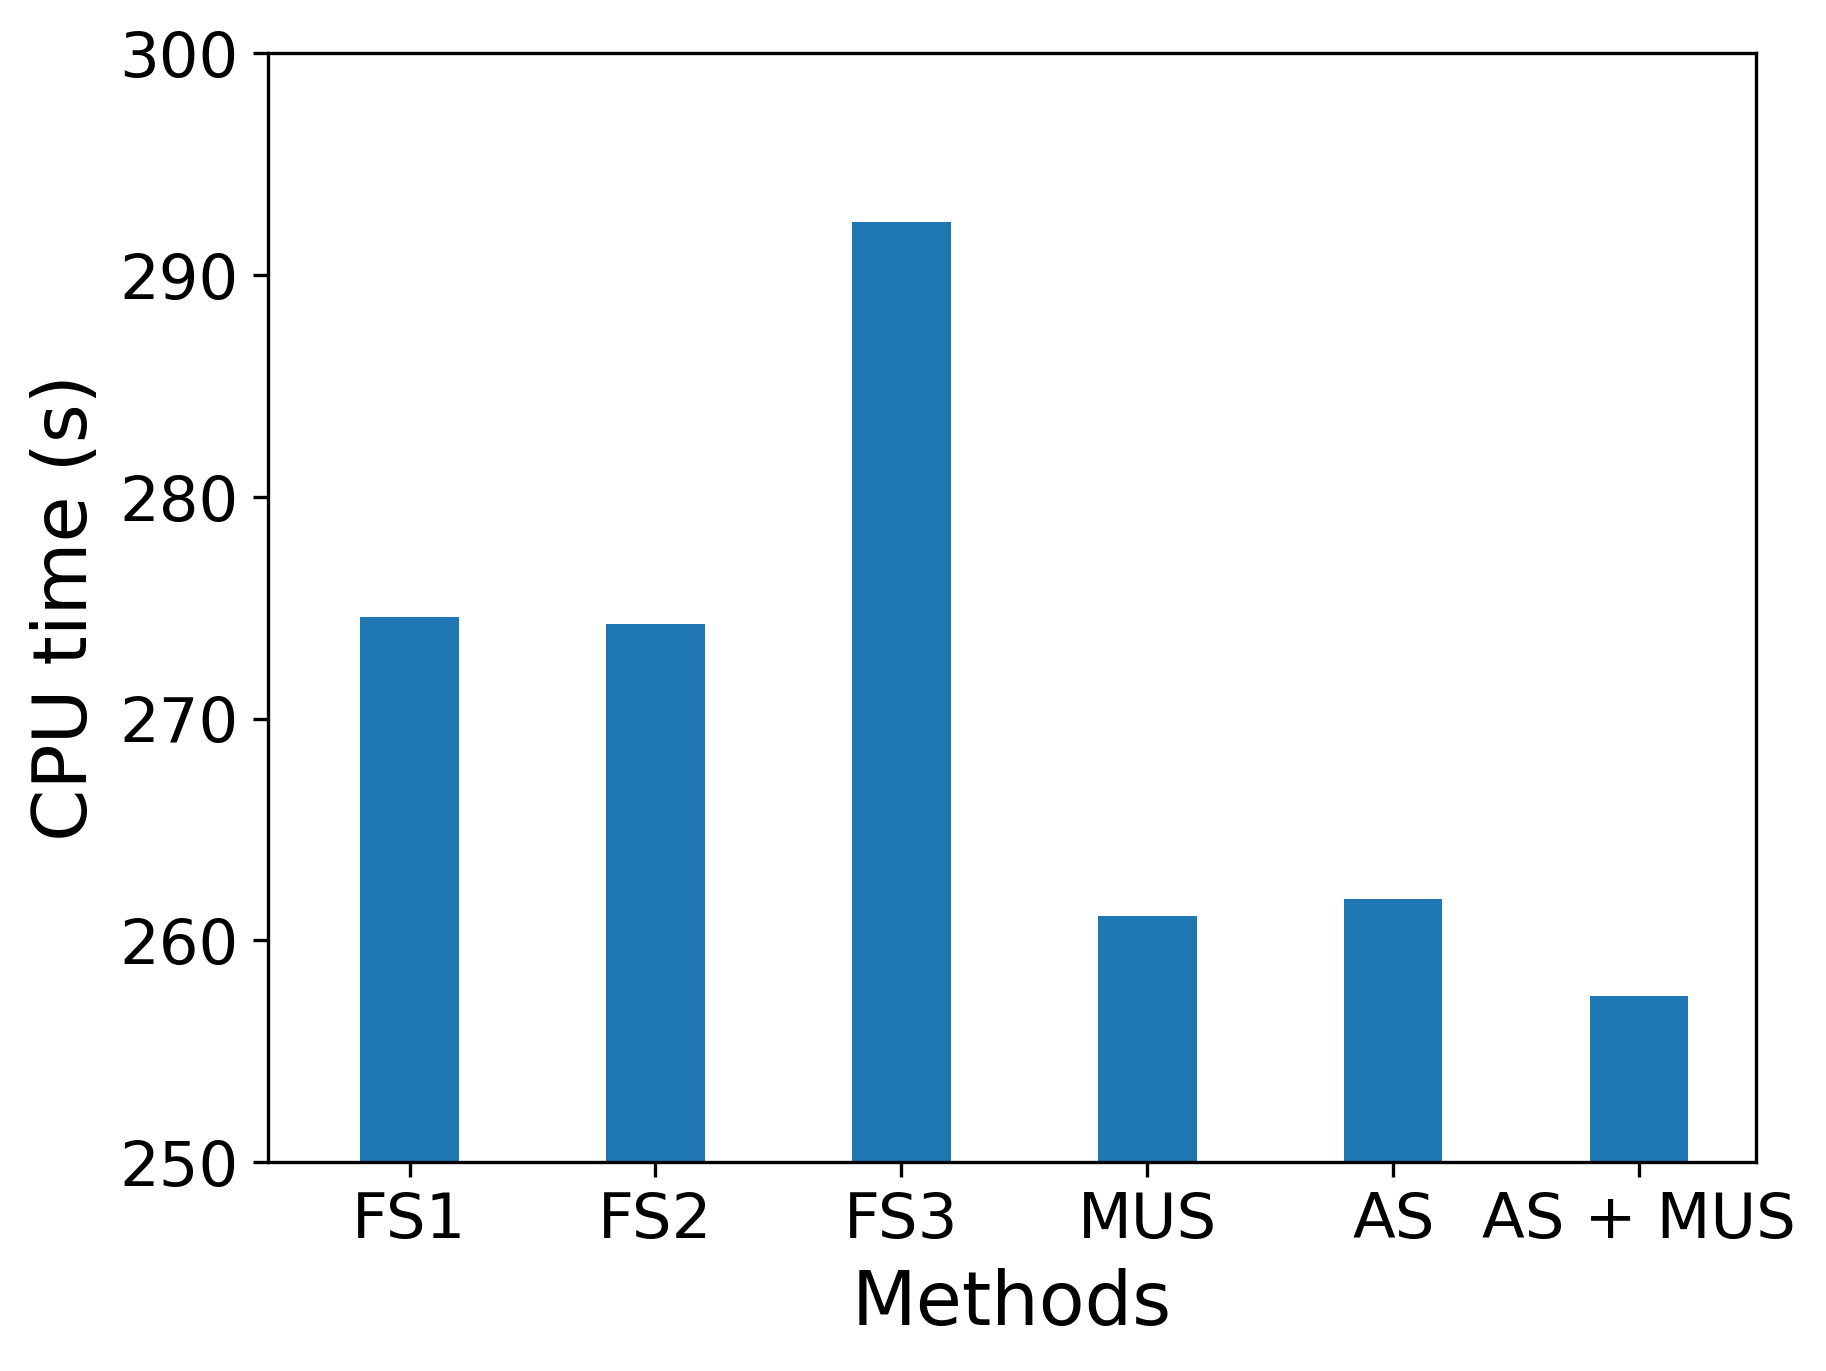
\includegraphics[width=0.45\linewidth]{llist.png}
\caption{Comparison between redundant records deletion methods. The fixed maximum table size method (FS) only removes data when the table is full, and the least recently used record is removed. The maximum table sizes for the 3 settings are, FS1: 140000, FS2: 130000, and FS3:120000. The maximum unused step method (MUS), removes records that haven't been used for a given number of time steps. 80 time steps are used for MUS. The adaptive maximum table size method (AS) used Eq.~\ref{eq:adap} to determine maximum table size, and $C=5.8, M=5$}
\label{droplet_delete} 
\end{figure}



%%%%%%%%%%%%%%%%%%%%%%%%%%%%%%%%%%%%%%%%%%%%%%%%%%%%%%%%%%%%%%%%%%%%%%%%%%%%%%%%
